\chapter{Metrics and Comparison}
\label{ch:results}

This chapter reports five experiments and the diagnostics that accompany them. Experiment~1 is a
preliminary run on a pre-processed Anki extract (Section~\ref{sec:results-exp1}). Experiment~2 is the
main benchmark on 100 Anki users (Section~\ref{sec:results-exp2}). Experiment~3 is a full Duolingo
benchmark (Section~\ref{sec:results-exp3}). Experiment~4 adds the improved models v2, v3 and a gradient-boosted tree model to both benchmarks
(Section~\ref{sec:results-exp4}). Experiment~5 adds constant floors, three further Anki samples and the srs-benchmark protocol
(Section~\ref{sec:results-exp5}). Section~\ref{sec:results-cross} compares the datasets. The remaining sections cover the MCMC diagnostics, the Task~3 sampler study, the
computational cost, and a summary. Section~\ref{sec:results-metrics} defines the metrics used
throughout. Every model is evaluated in the same way: it predicts each scored review from the
history before that review, and the predictions are scored against the recorded outcome.

\section{Evaluation Metrics}
\label{sec:results-metrics}

Let $N$ be the number of scored reviews. For review $i$ a model gives a predicted probability of
recall $p_i \in [0,1]$, and the observed outcome is $y_i \in \{0,1\}$, with $y_i = 1$ for a recalled
review. The rule that turns a raw grade or probability into $y_i$ is set by each dataset
(Chapter~\ref{ch:dataset}). The metrics below score the predictions from different angles, because a
model can rank reviews well and still be badly calibrated.

Log loss is the mean negative log likelihood of the outcomes under the predictions,
\begin{equation}\label{eq:logloss}
  \mathrm{LL} = -\frac{1}{N}\sum_{i=1}^{N}\bigl[\,y_i\log p_i + (1-y_i)\log(1-p_i)\,\bigr],
\end{equation}
where each $p_i$ is clipped to $[10^{-6},\, 1-10^{-6}]$ so that the logarithm is finite. Lower is
better. The Brier score is the mean squared error of the probabilities,
\begin{equation}\label{eq:brier}
  \mathrm{BS} = \frac{1}{N}\sum_{i=1}^{N}(p_i - y_i)^2,
\end{equation}
and is also lower-is-better. The area under the ROC curve (AUC) measures ranking only. It is the
probability that a randomly chosen recalled review receives a higher prediction than a randomly chosen
forgotten one,
\begin{equation}\label{eq:auc}
  \mathrm{AUC} = \frac{R_1 - n_1(n_1+1)/2}{n_1\, n_0},
\end{equation}
where $n_1$ and $n_0$ are the numbers of recalled and forgotten reviews, and $R_1$ is the sum of the
ranks of the recalled reviews' predictions among all $N$ predictions, with tied predictions given their
average rank. A constant predictor scores $0.5$, and higher is better.

The calibration metrics bin the predictions into equal-width intervals. For bin $b$, let $n_b$ be
the number of reviews, $\bar p_b$ the mean prediction, and $\bar y_b$ the observed recall rate. The
expected calibration error uses ten bins,
\begin{equation}\label{eq:ece}
  \mathrm{ECE} = \sum_{b=1}^{10}\frac{n_b}{N}\,\bigl|\bar y_b - \bar p_b\bigr|,
\end{equation}
and the root mean squared error over bins uses twenty bins, following the srs-benchmark convention,
\begin{equation}\label{eq:rmse}
  \mathrm{RMSE}_{\mathrm{bins}} = \Bigl(\sum_{b=1}^{20}\frac{n_b}{N}\bigl(\bar y_b - \bar p_b\bigr)^2\Bigr)^{1/2}.
\end{equation}
ECE and RMSE$_{\mathrm{bins}}$ are lower-is-better. The mean bias is the average prediction minus the
average outcome,
\begin{equation}\label{eq:bias}
  \bar b = \frac{1}{N}\sum_{i=1}^{N}(p_i - y_i) = \bar p - \bar y,
\end{equation}
so a positive value means the model is too optimistic overall. The reliability diagram plots
$\bar y_b$ against $\bar p_b$ for bins that contain at least 20 reviews. A calibrated model lies on
the diagonal.

Differences between models are tested with a paired, user-clustered bootstrap. Reviews from the same
user are correlated, so resampling single reviews would give intervals that are too narrow. Instead
users are drawn with replacement, all of a drawn user's reviews come along, and the same users are
used for both models. For a metric $M$ and two models,
\begin{equation}\label{eq:boot}
  \Delta = M(\text{model}) - M(\text{reference}), \qquad
  \mathrm{CI}_{95} = \bigl[\,q_{\alpha/2}(\Delta^{*}),\; q_{1-\alpha/2}(\Delta^{*})\,\bigr],
\end{equation}
where $\Delta^{*}$ is the difference recomputed on each of 1000 resamples of users (seed 0),
$q_{\alpha/2}$ and $q_{1-\alpha/2}$ are the corresponding quantiles of those values, and $\alpha$ is
one minus the confidence level. A difference is called significant only when its interval excludes zero. In the tables that report intervals, an asterisk marks such intervals. Intervals
that include zero are reported as not significant.

\section{Experiment 1: Preliminary Anki Run}
\label{sec:results-exp1}

Experiment~1 is a preliminary run, and it is reported as such. It uses a pre-processed Anki extract with
separate training and test files. The extract has 20,000 card sequences and 52,937 test reviews, and
the overall test recall is 0.858. The median gap between reviews is 5 days, the 90th percentile is 38
days, and the longest gap is 2149 days. The provenance of this extract has not been fully
authenticated, and the sampler was run for only 200 iterations as a single chain. The learned rate has
posterior mean 0.393 with an interval of [0.339, 0.471], an effective sample size of 3, and split
$\hat R = 2.09$. The chain had therefore not converged, and the numbers below describe one short run.

Five models are compared on five gap bins (0--1\,d, 1--3\,d, 3--14\,d, 14--60\,d and 60\,d+). The bins
are those of Experiment~1 and differ from the bins of Experiment~2. LagLogit+$\Delta t$ is a static
logistic model whose inputs are the lagged outcome and the gap. HLR is included as a trainable baseline.
The dynamic model, labelled Dyn in the figures and tables, appears in four forms: with the learned
rate, with the rate fixed near zero (no decay), with the rate fixed at 5 (no memory), and with the
practice coefficient $\kappa$ free. The last three are ablations. They test whether the decay and the
latent state carry information about recall.

Table~\ref{tab:exp1-gap} gives the log loss in each bin, and Figure~\ref{fig:fig_exp1_gap_logloss}
plots the same values. The bold entries show that no single model is best everywhere. LagLogit+$\Delta t$
is best in the 0--1\,d bin, the no-memory variant is best in the 1--3\,d and 3--14\,d bins, HLR is best
in the 14--60\,d bin, and the no-decay variant is best in the 60\,d+ bin. The learned-rate model is never
the best in a bin. HLR's log loss of 2.241 in the 0--1\,d bin is far above the others. The bias in that
bin is +0.243 and its AUC is 0.500, which is chance level, so the HLR value is shown off scale in the
figure. The 60\,d+ bin is the hardest for LagLogit+$\Delta t$ and for the learned-rate model, where it has
the highest log loss of their five bins.

\begin{table}[htbp]
  \centering
  \caption[Experiment 1: log loss by gap bin]{Experiment 1: log loss by gap bin (lower is better). Bold marks the lowest value in each
    column. Source: \texttt{AnkiFirstRun/anki\_second\_run.txt}.}
  \label{tab:exp1-gap}
  \begin{tabular}{@{}lccccc@{}}
    \toprule
    Model & 0--1\,d & 1--3\,d & 3--14\,d & 14--60\,d & 60\,d+ \\
    \midrule
    LagLogit+$\Delta t$ & \textbf{0.371} & 0.345 & 0.350 & 0.346 & 0.472 \\
    HLR & 2.241 & 0.492 & 0.368 & \textbf{0.266} & 0.696 \\
    Dyn learned-$\lambda$ & 0.405 & 0.329 & 0.337 & 0.273 & 0.420 \\
    Dyn $\lambda\approx0$ (no decay) & 0.441 & 0.397 & 0.338 & 0.283 & \textbf{0.401} \\
    Dyn $\lambda=5$ (no memory) & 0.398 & \textbf{0.325} & \textbf{0.332} & 0.285 & 0.440 \\
    Dyn $+\kappa$ & 0.402 & 0.328 & 0.335 & 0.272 & 0.421 \\
    \bottomrule
  \end{tabular}
\end{table}

\begin{figure}[htbp]
  \centering
  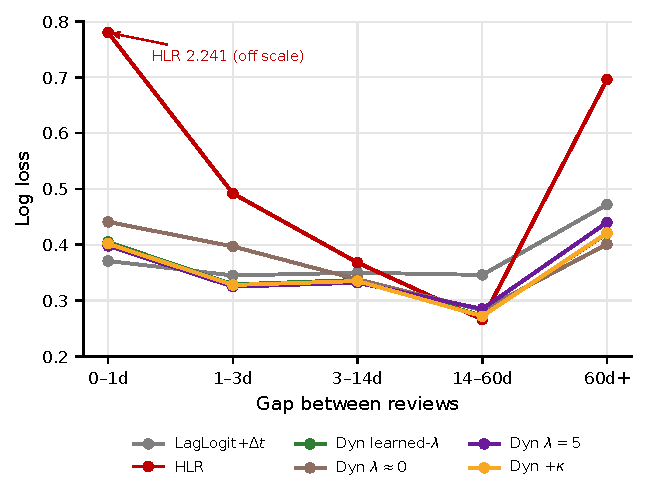
\includegraphics[width=\textwidth]{figures/data/fig_exp1_gap_logloss.pdf}
  \caption[Experiment 1: log loss by gap bin]{Experiment 1: log loss by gap bin for LagLogit+$\Delta t$, HLR and the four dynamic variants.
    The HLR value in the 0--1\,d bin (2.241) is off scale and labelled. Apart from HLR, the curves lie
    close together, and for LagLogit+$\Delta t$ and the learned-rate model the longest bin is the
    highest point of the curve.}
  \label{fig:fig_exp1_gap_logloss}
\end{figure}

Calibration is shown in Figure~\ref{fig:fig_exp1_gap_bias}, which plots the mean bias in each bin. A
bias near zero is good. LagLogit+$\Delta t$ under-predicts recall in the 14--60\,d bin, with a bias of
$-0.155$. The learned-rate model reduces that bias to $-0.051$, which is about 67\% smaller in magnitude
in the preliminary run. At 60\,d and longer, the learned-rate model over-predicts, with a bias of
$+0.075$, and the no-decay variant is close to zero there.

\begin{figure}[htbp]
  \centering
  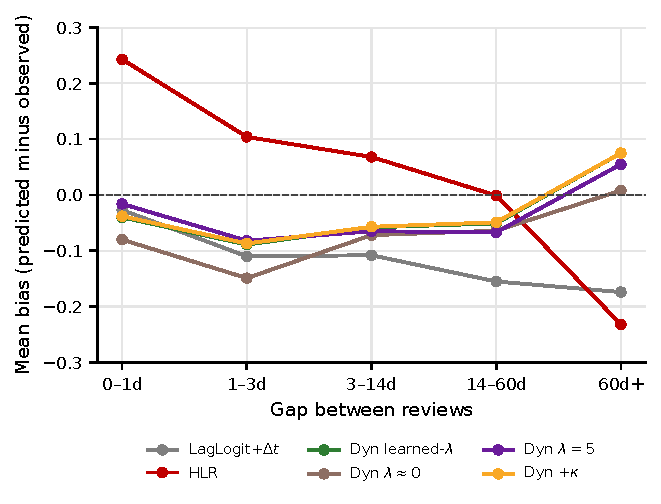
\includegraphics[width=\textwidth]{figures/data/fig_exp1_gap_bias.pdf}
  \caption[Experiment 1: mean bias by gap bin]{Experiment 1: mean bias (mean prediction minus observed recall) by gap bin, for the six
    models. Zero is marked by the dashed line. HLR is most optimistic in the shortest bin and the
    learned-rate model is closest to zero in the middle bins.}
  \label{fig:fig_exp1_gap_bias}
\end{figure}

The paired comparison in Table~\ref{tab:exp1-paired} asks whether the learned-rate model differs from
LagLogit+$\Delta t$ in each bin. The difference is significant in two bins. In the 0--1\,d bin the
learned-rate model is worse, with an interval entirely above zero. In the 14--60\,d bin it is better,
with an interval entirely below zero. The other three intervals include zero. Figure~\ref{fig:fig_exp1_paired_forest}
shows the same comparison for all four dynamic variants. The four variants overlap closely in each bin,
and their intervals are wide. The overall ablations, which pool all bins, are in Table~\ref{tab:exp1-ablation}.

\begin{table}[htbp]
  \centering
  \caption[Experiment 1: paired log-loss differences]{Experiment 1: paired difference in log loss, learned-$\lambda$ model minus
    LagLogit+$\Delta t$, by gap bin. Negative values favour the learned-$\lambda$ model. Asterisks
    mark intervals that exclude zero. Bold marks the most favourable value.}
  \label{tab:exp1-paired}
  \begin{tabular}{@{}lcc@{}}
    \toprule
    Gap bin & $\Delta$ log loss & 95\% interval \\
    \midrule
    0--1\,d & $+0.0333$ & $[+0.0107,\ +0.1115]^{*}$ \\
    1--3\,d & $-0.0162$ & $[-0.0332,\ +0.0123]$ \\
    3--14\,d & $-0.0129$ & $[-0.0654,\ +0.0132]$ \\
    14--60\,d & \textbf{$-0.0735$} & $[-0.1032,\ -0.0573]^{*}$ \\
    60\,d+ & $-0.0525$ & $[-0.1390,\ +0.0270]$ \\
    \bottomrule
  \end{tabular}
\end{table}

\begin{figure}[htbp]
  \centering
  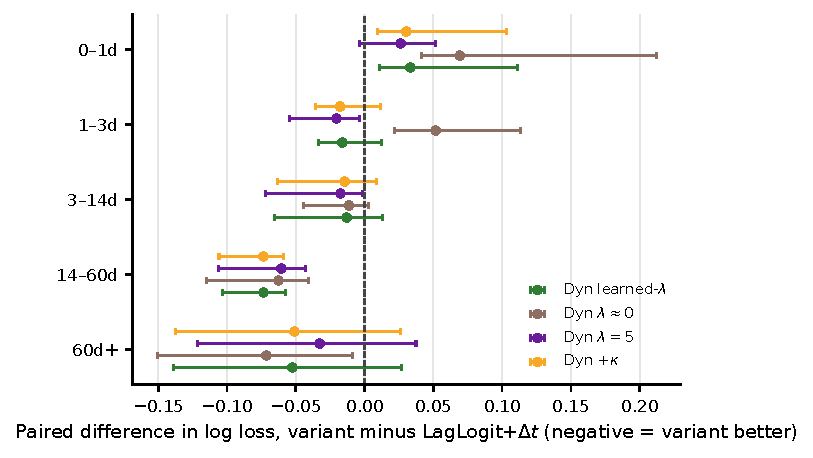
\includegraphics[width=\textwidth]{figures/data/fig_exp1_paired_forest.pdf}
  \caption[Experiment 1: paired differences by gap bin]{Experiment 1: paired differences in log loss, each dynamic variant minus LagLogit+$\Delta t$,
    with 95\% intervals, by gap bin. Points left of the dashed line favour the variant. The four
    variants are offset vertically within each bin so that their intervals can be read separately.}
  \label{fig:fig_exp1_paired_forest}
\end{figure}

The overall ablations are in Table~\ref{tab:exp1-ablation}. Each row is a variant minus the learned-rate
model. Removing the decay (rate near zero) makes log loss worse by 0.0199, and that interval excludes
zero, so in this run the decay carries information. The no-memory variant (rate fixed at 5) is
indistinguishable from the learned rate, with a difference of 0.0000 and an interval that includes zero.
The practice coefficient $\kappa$ moves log loss by $-0.0014$, which is not significant.

\begin{table}[htbp]
  \centering
  \caption[Experiment 1: overall ablation]{Experiment 1: overall ablation. Each row is a variant minus the learned-$\lambda$ model, in
    log loss, with its 95\% interval. Positive values mean the variant is worse. Asterisks mark
    intervals that exclude zero. Bold marks the lowest value, which is not significant.}
  \label{tab:exp1-ablation}
  \begin{tabular}{@{}lcc@{}}
    \toprule
    Variant & $\Delta$ log loss & 95\% interval \\
    \midrule
    No decay ($\lambda\approx0$) & $+0.0199$ & $[+0.0031,\ +0.0343]^{*}$ \\
    No memory ($\lambda=5$) & $+0.0000$ & $[-0.0181,\ +0.0071]$ \\
    Free $\kappa$ & \textbf{$-0.0014$} & $[-0.0041,\ +0.0003]$ \\
    \bottomrule
  \end{tabular}
\end{table}

The interim update reported an overall calibration error (ECE) for these models, computed from its
reliability plot rather than from the run log. The values were 0.050 for the learned-rate model, 0.105
for LagLogit+$\Delta t$, 0.108 for HLR and 0.082 for the no-decay variant. These are the only ECE
values for Experiment~1 in this report, and they were not recomputed here.

Taken together, Experiment~1 is consistent with the dynamic model helping in the 14--60\,d bin, where
it has lower log loss and a smaller bias than LagLogit+$\Delta t$. It is worse in the 0--1\,d bin, and
its AUC is lower than that of LagLogit+$\Delta t$ in three bins, by 0.020 in the 0--1\,d bin, 0.096
in the 3--14\,d bin and 0.039 in the 14--60\,d bin. Those three AUC differences exclude zero. HLR has the
lowest log loss at 14--60 days, and the no-memory variant matches the learned rate overall. The sample
is small, the chain did not converge, and the provenance of the data is not authenticated. Experiment~1
therefore motivates the larger benchmark in Section~\ref{sec:results-exp2}, and it is not evidence for
the model on its own.

\section{Experiment 2: FSRS Benchmark}
\label{sec:results-exp2}

Experiment~2 is the main benchmark on Anki data. It uses 100 users from the public
\texttt{anki-revlogs-10k} collection \cite{ankirevlogs10k}, sampled with seed 0, with at most 1000
cards per user. The sample contains 99,074 cards and 768,658 review events. For each user the cutoff is
the 80th percentile of that user's day offsets. Reviews before the cutoff form the training data (606,364
events), and later reviews form the test data (162,294 events). A test review is scored only if it is not
the card's first review and its elapsed time is at least one day. This leaves 95,400 scored reviews, of
which 0.831 are recalls. Every model is fitted on the training events and predicts each scored review
from the history before it.

Five models are compared. FSRS-6 with default weights uses the py-fsrs implementation \cite{pyfsrs} with
its 21 default parameters. FSRS-6 with optimised weights fits those parameters per user on the training
data, and falls back to the defaults for one user who has too few informative training reviews. HLR is a
port of Duolingo's official code \cite{settles2016trainable}. The proposed model is shown with its learned
rate and with the practice coefficient $\kappa$ free. FSRS-6 uses all four Anki grades, whereas the
proposed model uses a binary outcome: a review counts as recalled if its grade is above Again. The
proposed model therefore receives less information than FSRS-6 does, and this should be kept in mind when
the results are read. The proposed model's chain did not converge (Section~\ref{sec:results-mcmc}), so its
scores are provisional.

Table~\ref{tab:exp2-overall} gives the overall metrics, and Figure~\ref{fig:fig_overall_bars} plots three of
them. Among the five models of Experiment 2, FSRS-6 with optimised weights is the best model on every metric in the table. Its log loss is 0.379
against 0.396 for FSRS-6 with default weights, its AUC is 0.777, and its ECE is 0.009. The proposed model
ranks third on log loss (0.422) and fourth on AUC (0.692), and its learned-rate and $\kappa$ variants are almost
identical. Among these five models, HLR is the weakest, with the highest log loss (0.680), the lowest AUC (0.555), and the
highest ECE (0.146). Its mean bias is also the largest, at +0.060.

\begin{table}[htbp]
  \centering
  \caption[Experiment 2: overall metrics]{Experiment 2: overall metrics on the 95,400 scored reviews. Log loss, Brier, ECE, RMSE$_{\mathrm{bins}}$
    and the absolute value of the mean bias are lower-is-better, and AUC is higher-is-better. Bold marks the best
    value in each column; for the mean bias, the best value is the one closest to zero.}
  \label{tab:exp2-overall}
  \begin{tabular}{@{}lcccccc@{}}
    \toprule
    Model & Log loss & Brier & AUC & ECE & RMSE$_{\mathrm{bins}}$ & Mean bias \\
    \midrule
    FSRS-6 (default) & 0.396 & 0.121 & 0.745 & 0.012 & 0.017 & $+0.011$ \\
    FSRS-6 (optimised) & \textbf{0.379} & \textbf{0.117} & \textbf{0.777} & \textbf{0.009} & \textbf{0.014} & \textbf{$-0.002$} \\
    HLR & 0.680 & 0.170 & 0.555 & 0.146 & 0.176 & $+0.060$ \\
    Ours (learned $\lambda$) & 0.422 & 0.131 & 0.692 & 0.025 & 0.032 & $+0.011$ \\
    Ours ($+\kappa$) & 0.422 & 0.131 & 0.693 & 0.026 & 0.032 & $+0.011$ \\
    \bottomrule
  \end{tabular}
\end{table}

\begin{figure}[htbp]
  \centering
  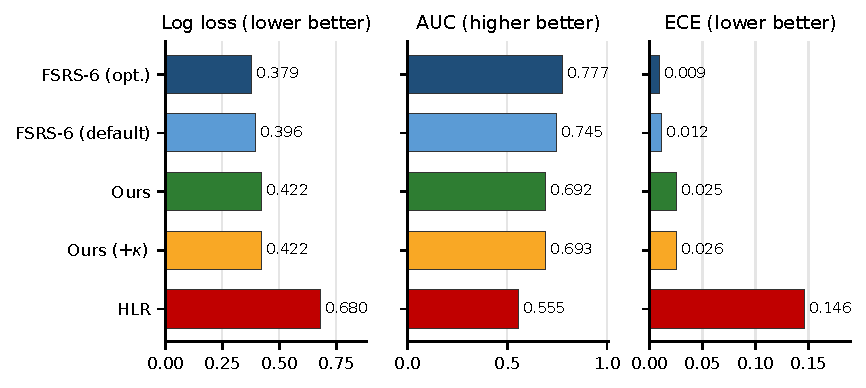
\includegraphics[width=\textwidth]{figures/data/fig_overall_bars.pdf}
  \caption[Experiment 2: overall metrics]{Experiment 2: overall log loss, AUC and ECE for the five models, on 95,400 scored reviews.
    Each bar starts at zero. The FSRS-6 (optimised) bars are the lowest for log loss and ECE and the
    highest for AUC. The HLR bars are the tallest for log loss and ECE and the shortest for AUC.}
  \label{fig:fig_overall_bars}
\end{figure}

The gap between reviews matters, so Table~\ref{tab:exp2-gap} and Figure~\ref{fig:fig_gap_logloss} split
the log loss by gap bin. The bins are 1 day, 2--3 days, 4--14 days, 15--60 days and 61 days or more.
The model order is the same in every bin: FSRS-6 (optimised) is best, followed by FSRS-6 (default), the
proposed model and HLR. HLR changes the most with the gap. Its log loss is 0.942 at one day, falls to
0.473 at 15--60 days, and rises to 0.771 at 61 days or more. The other models are much flatter across the
bins, and the proposed model's log loss stays between 0.398 and 0.460 across all five bins.

\begin{table}[htbp]
  \centering
  \caption[Experiment 2: log loss by gap bin]{Experiment 2: log loss by gap bin. Bold marks the lowest value in each column. The
    proposed model with $\kappa$ free equals the learned-rate model to three decimals in every bin.}
  \label{tab:exp2-gap}
  \begin{tabular}{@{}lccccc@{}}
    \toprule
    Model & 1\,d & 2--3\,d & 4--14\,d & 15--60\,d & 61\,d+ \\
    \midrule
    FSRS-6 (default) & 0.409 & 0.402 & 0.369 & 0.401 & 0.418 \\
    FSRS-6 (optimised) & \textbf{0.396} & \textbf{0.389} & \textbf{0.361} & \textbf{0.374} & \textbf{0.389} \\
    HLR & 0.942 & 0.734 & 0.555 & 0.473 & 0.771 \\
    Ours (learned $\lambda$) & 0.423 & 0.426 & 0.398 & 0.419 & 0.460 \\
    Ours ($+\kappa$) & 0.423 & 0.426 & 0.398 & 0.419 & 0.460 \\
    \bottomrule
  \end{tabular}
\end{table}

\begin{figure}[htbp]
  \centering
  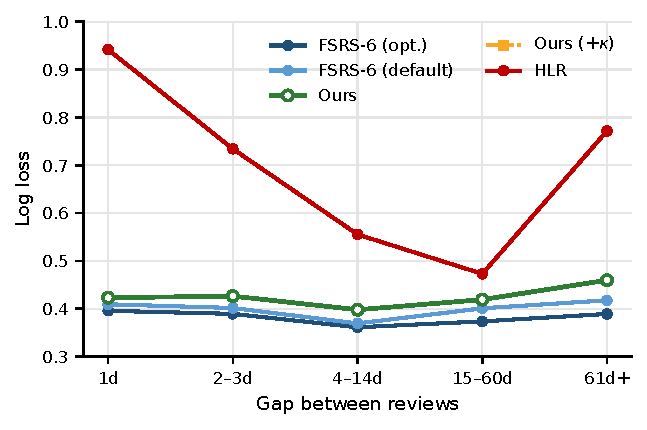
\includegraphics[width=\textwidth]{figures/data/fig_gap_logloss.pdf}
  \caption[Experiment 2: log loss by gap bin]{Experiment 2: log loss by gap bin for the five models. The FSRS-6 (optimised) line is lowest in
    every bin. The HLR line is steep at short gaps and falls to its lowest point at 15--60 days.}
  \label{fig:fig_gap_logloss}
\end{figure}

Calibration by gap is shown in Figure~\ref{fig:fig_gap_bias}. HLR over-predicts recall at short gaps,
with a bias of $+0.170$ at one day, and under-predicts at 61 days and longer, with a bias of $-0.249$.
The proposed model is almost unbiased at one day ($-0.006$) but over-predicts at 61 days and longer,
with a bias of $+0.090$. This is an honest limitation: the proposed model does not remove the long-gap
error in this benchmark.

\begin{figure}[htbp]
  \centering
  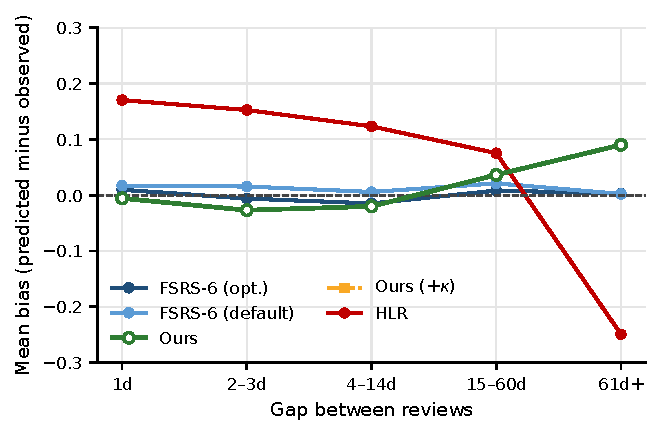
\includegraphics[width=\textwidth]{figures/data/fig_gap_bias.pdf}
  \caption[Experiment 2: mean bias by gap bin]{Experiment 2: mean bias by gap bin (predicted minus observed recall), for the five models. Ours and Ours (+$\kappa$) nearly coincide, so the second is largely hidden under the first. The
    dashed line marks zero. HLR moves from strongly optimistic to strongly pessimistic across the bins,
    while the proposed model is close to zero in the shorter bins and is most optimistic in the longest bin.}
  \label{fig:fig_gap_bias}
\end{figure}

Figure~\ref{fig:fig_reliability} shows the reliability diagram. The FSRS-6 curves lie close to the
diagonal. The proposed model sits above the diagonal in the middle of the range, which means it
under-predicts recall there. In the bin around 0.5--0.6 it predicts 0.555 on average, but 0.629 of those
reviews are recalled. HLR is far from the diagonal across the whole range, and at low predicted
probabilities the observed recall is much higher than predicted.

\begin{figure}[htbp]
  \centering
  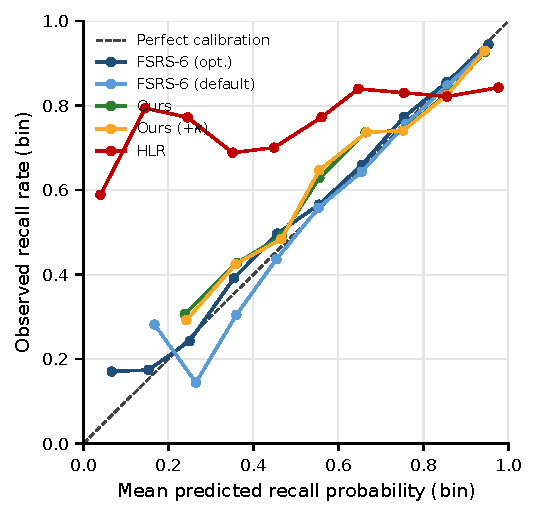
\includegraphics[width=12cm]{figures/data/fig_reliability.pdf}
  \caption[Experiment 2: reliability diagram]{Experiment 2: reliability diagram on the scored reviews. Each point is a bin of predicted
    probability with at least 20 reviews, plotted at its mean prediction (horizontal) and observed recall
    rate (vertical). The dashed diagonal is perfect calibration.}
  \label{fig:fig_reliability}
\end{figure}

The paired comparison is in Figure~\ref{fig:fig_paired_forest}. The proposed model has a higher log loss
than FSRS-6 with optimised weights, by 0.043 (interval [0.033, 0.055]), and than FSRS-6 with default
weights, by 0.026 (interval [0.013, 0.042]). Both intervals exclude zero, so these are significant
differences that favour FSRS-6. Against HLR the proposed model is better, with a difference of $-0.258$
(interval [$-0.314$, $-0.204$]). The AUC differences point the same way. The proposed model's AUC is lower
than FSRS-6 (optimised) by 0.084 and than FSRS-6 (default) by 0.053, and higher than HLR by 0.137, and all
those intervals exclude zero. The $\kappa$ variant does not differ from the learned-rate model. Its
difference is $-0.0002$ in log loss, with an interval of [$-0.0008$, $+0.0004$]. The forest plot therefore
shows that row as zero to three decimals.

\begin{figure}[htbp]
  \centering
  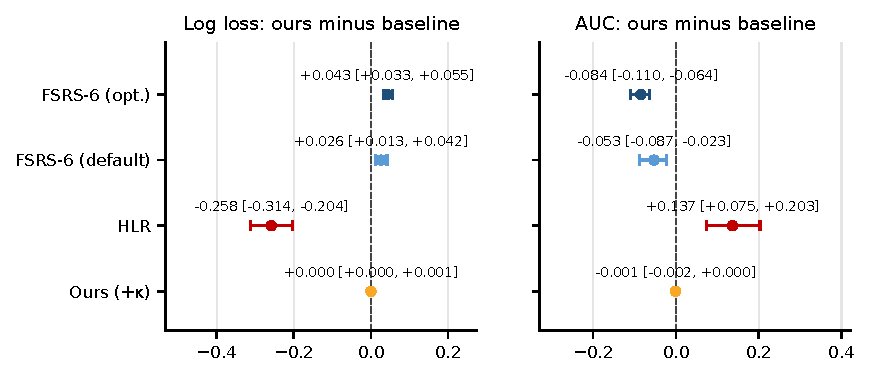
\includegraphics[width=\textwidth]{figures/data/fig_paired_forest.pdf}
  \caption[Experiment 2: paired differences]{Experiment 2: paired differences, the proposed model minus each comparison model, with 95\%
    user-clustered bootstrap intervals (1000 resamples). Left: log loss. Right: AUC. The dashed line marks
    zero. The last row is the learned-rate model minus the $\kappa$ variant, so it is the negative of the
    difference quoted in the text.}
  \label{fig:fig_paired_forest}
\end{figure}

The per-user comparison in Figure~\ref{fig:fig_user_wins} gives the same picture. For each user the mean
log loss over that user's scored reviews is computed, and the number of users for whom one model is lower
is counted. FSRS-6 with optimised weights has the lower per-user log loss for 78 of the 100 users, FSRS-6
with default weights for 68, and the proposed model beats HLR for 86. The $\kappa$ variant beats the
learned-rate model for 52 users, which is close to an even split.

\begin{figure}[htbp]
  \centering
  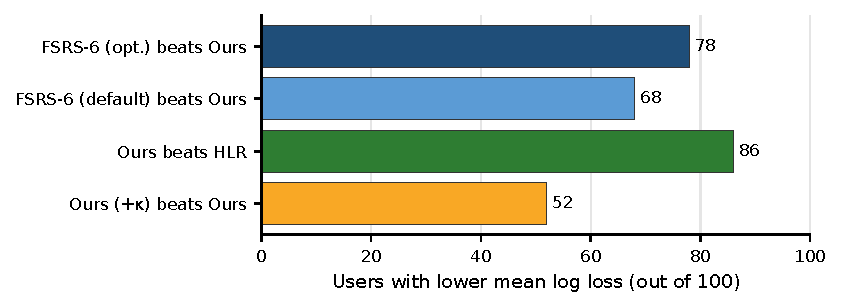
\includegraphics[width=12cm]{figures/data/fig_user_wins.pdf}
  \caption[Experiment 2: users with lower log loss]{Experiment 2: number of the 100 users for whom the first model has lower mean log loss than the
    second. Read each bar as a count out of 100, and see the labels for the comparison.}
  \label{fig:fig_user_wins}
\end{figure}

Figure~\ref{fig:fig_user_scatter} puts the same per-user log losses on a scatter plot, with FSRS-6
(optimised) on the horizontal axis and the proposed model on the vertical axis. Points above the dashed
diagonal are users for whom FSRS-6 predicts better. Most points lie above the diagonal, which matches the
count of 78 users. A small number of users lie far above the diagonal, at high log loss for the proposed model.

\begin{figure}[htbp]
  \centering
  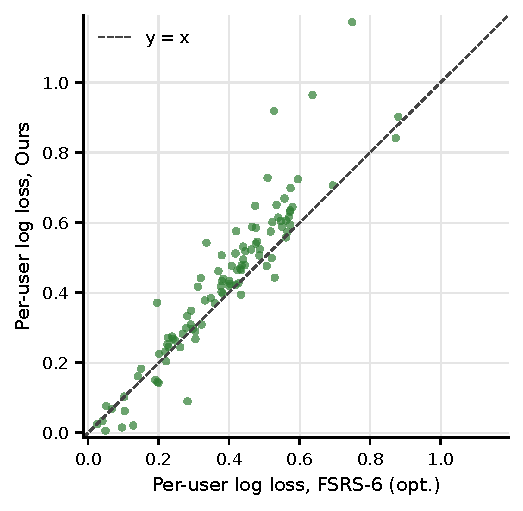
\includegraphics[width=12cm]{figures/data/fig_user_scatter.pdf}
  \caption[Experiment 2: per-user log loss]{Experiment 2: per-user mean log loss, FSRS-6 (optimised) against the proposed model. Each point is
    one user. Points above the dashed line are users for whom FSRS-6 predicts better.}
  \label{fig:fig_user_scatter}
\end{figure}

Cards are split into warm and cold cards. A warm card has training reviews, and its state starts from the
last training draw. A cold card has none, so at each test review the prediction starts again from the prior
(Section~\ref{sec:method-prediction}). Cold cards are 41,469 of the 95,400 scored reviews (43.5\%), and
warm cards are 53,931. Figure~\ref{fig:fig_warm_cold} shows that FSRS-6 is better on both groups.
The proposed model is in fact slightly better on cold cards than on warm cards in log loss (0.417 against
0.426), but its AUC is lower on cold cards (0.684 against 0.699). Its gap to FSRS-6 (optimised) is slightly
larger on cold cards: log loss is 0.417 against 0.372 on cold cards and 0.426 against 0.385 on warm cards,
and AUC is 0.684 against 0.781 on cold cards and 0.699 against 0.774 on warm cards. The cold path therefore
does not by itself explain the gap to FSRS-6, which is present on both groups. It is a limitation of the
implementation, because it uses less of each card's history than it could. Chapter~\ref{ch:conclusion} returns to this point.

\begin{figure}[htbp]
  \centering
  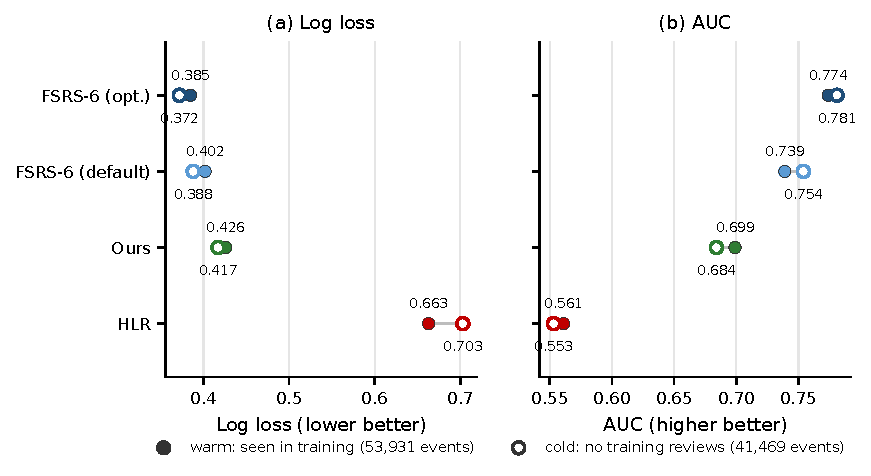
\includegraphics[width=\textwidth]{figures/data/fig_warm_cold.pdf}
  \caption[Experiment 2: warm and cold cards]{Experiment 2: log loss and AUC for warm cards (filled markers, 53,931 reviews) and cold cards
    (open markers, 41,469 reviews), per model. A grey line joins the two values for each model. Cold
    cards have no training reviews.}
  \label{fig:fig_warm_cold}
\end{figure}

On the Anki benchmark, among the five models of Experiment 2, FSRS-6 with optimised weights is the best model on every metric, and the proposed
model is better than HLR but worse than both FSRS-6 variants. These are the results of a single, unconverged
chain, so they are provisional. The diagnostics are discussed in Section~\ref{sec:results-mcmc}, and the
comparison with the Duolingo benchmark follows in Sections~\ref{sec:results-exp3} and~\ref{sec:results-cross}.

\section{Experiment 3: Full Duolingo}
\label{sec:results-exp3}

Experiment~3 applies the same protocol to the full Duolingo half-life regression traces \cite{settles2016trainable}.
Its purpose is to test whether the Experiment~2 ranking holds on a much larger dataset with a different
outcome. Table~\ref{tab:exp3-setup} in Chapter~\ref{ch:dataset} summarises the setup. A card is a pair of user and lexeme. The outcome is
binary: a review is recalled if the predicted recall probability in the trace is at least 0.5. FSRS-6 therefore
sees only two outcomes, Again and Good, and not the four Anki grades. The split and scoring follow
Section~\ref{sec:results-exp2}.


Table~\ref{tab:exp3-overall} gives the overall metrics, and Figure~\ref{fig:fig_exp3_overall_bars} plots them.
The proposed model is the best of the five models on log loss, Brier score, AUC, ECE and RMSE over bins.
Its log loss is 0.268 against 0.300 for FSRS-6 (optimised) and 0.291 for LagLogit+$\Delta t$. Its AUC is 0.656,
against 0.570 for FSRS-6 (optimised) and 0.653 for LagLogit+$\Delta t$. The only metric on which it is not best is the
mean bias. There LagLogit+$\Delta t$ is closest to zero, at $-0.001$, while the proposed model's bias is $+0.004$.

\begin{table}[htbp]
  \centering
  \caption[Experiment 3: overall metrics]{Experiment 3: overall metrics on 1,189,355 scored reviews. Bold marks the
    best value in each column; for the mean bias, the best value is the one closest to zero.}
  \label{tab:exp3-overall}
  \begin{tabular}{@{}lcccccc@{}}
    \toprule
    Model & Log loss & Brier & AUC & ECE & RMSE$_{\mathrm{bins}}$ & Mean bias \\
    \midrule
    FSRS-6 (default) & 0.302 & 0.078 & 0.566 & 0.051 & 0.070 & $-0.025$ \\
    FSRS-6 (optimised) & 0.300 & 0.078 & 0.570 & 0.050 & 0.070 & $-0.026$ \\
    HLR & 0.418 & 0.079 & 0.521 & 0.072 & 0.072 & $+0.072$ \\
    LagLogit+$\Delta t$ & 0.291 & 0.076 & 0.653 & 0.020 & 0.068 & \textbf{$-0.001$} \\
    Ours (GPU) & \textbf{0.268} & \textbf{0.071} & \textbf{0.656} & \textbf{0.014} & \textbf{0.017} & $+0.004$ \\
    \bottomrule
  \end{tabular}
\end{table}

\begin{figure}[htbp]
  \centering
  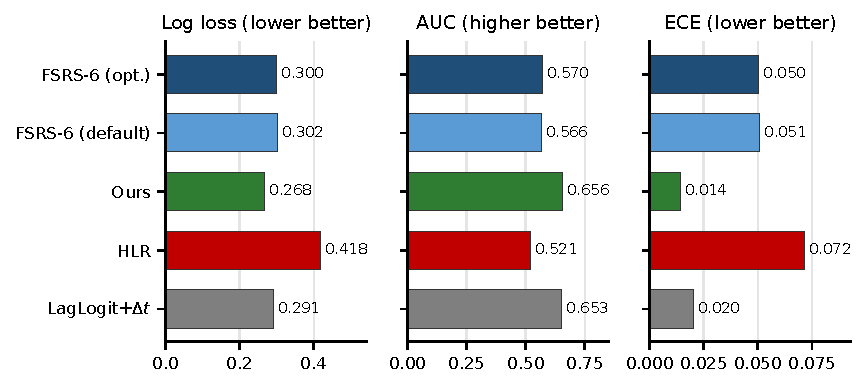
\includegraphics[width=\textwidth]{figures/data/fig_exp3_overall_bars.pdf}
  \caption[Experiment 3: overall metrics]{Experiment 3: overall log loss, AUC and ECE for the five models on full
    Duolingo. Each bar starts at zero. The proposed model has the shortest log-loss and ECE bars and the longest AUC
    bar, although its AUC is only slightly above that of LagLogit+$\Delta t$.}
  \label{fig:fig_exp3_overall_bars}
\end{figure}

The gap structure is shown in Table~\ref{tab:exp3-gap} and Figure~\ref{fig:fig_exp3_gap_logloss}. Only three gap bins
contain scored reviews, so the figure has three points per line. In every bin the proposed model has the lowest
log loss, from 0.261 at one day to 0.275 at 4--14 days. The AUC ordering is not uniform. The proposed model is best at
one day and 2--3 days, but at 4--14 days LagLogit+$\Delta t$ has the highest AUC (0.658 against 0.655).

\begin{table}[htbp]
  \centering
  \caption[Experiment 3: log loss and AUC by gap]{Experiment 3: log loss and AUC by gap bin. Scored reviews:
    444,662 at one day, 376,692 at 2--3 days and 368,001 at 4--14 days. Bold marks the best value in each column.}
  \label{tab:exp3-gap}
  \begin{tabular}{@{}lcccccc@{}}
    \toprule
    & \multicolumn{3}{c}{Log loss} & \multicolumn{3}{c}{AUC} \\
    \cmidrule(lr){2-4}\cmidrule(lr){5-7}
    Model & 1\,d & 2--3\,d & 4--14\,d & 1\,d & 2--3\,d & 4--14\,d \\
    \midrule
    FSRS-6 (default) & 0.290 & 0.293 & 0.325 & 0.580 & 0.564 & 0.554 \\
    FSRS-6 (optimised) & 0.288 & 0.292 & 0.324 & 0.584 & 0.567 & 0.556 \\
    HLR & 0.481 & 0.407 & 0.353 & 0.543 & 0.530 & 0.522 \\
    LagLogit+$\Delta t$ & 0.290 & 0.291 & 0.292 & 0.652 & 0.650 & \textbf{0.658} \\
    Ours (GPU) & \textbf{0.261} & \textbf{0.270} & \textbf{0.275} & \textbf{0.660} & \textbf{0.652} & 0.655 \\
    \bottomrule
  \end{tabular}
\end{table}

\begin{figure}[htbp]
  \centering
  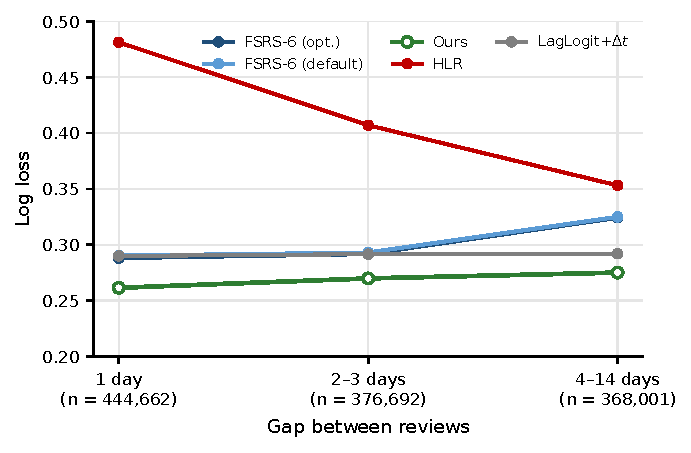
\includegraphics[width=\textwidth]{figures/data/fig_exp3_gap_logloss.pdf}
  \caption[Experiment 3: log loss by gap]{Experiment 3: log loss by gap bin for the five models. Only the three
    populated bins are shown, and the number of scored reviews is printed under each bin. The proposed model's line is the lowest in every bin.}
  \label{fig:fig_exp3_gap_logloss}
\end{figure}

Figure~\ref{fig:fig_exp3_reliability} shows the reliability diagram. Over the lower and middle range, all four curves lie above the diagonal, so observed recall is higher than predicted there. Near the top of the range the curves approach the diagonal. HLR appears as a single point at the top right,
because every one of its predictions falls in that bin and its other bins contain fewer than 20 reviews, so no
other point is drawn. Its mean bias is $+0.072$ (Table~\ref{tab:exp3-overall}).

\begin{figure}[htbp]
  \centering
  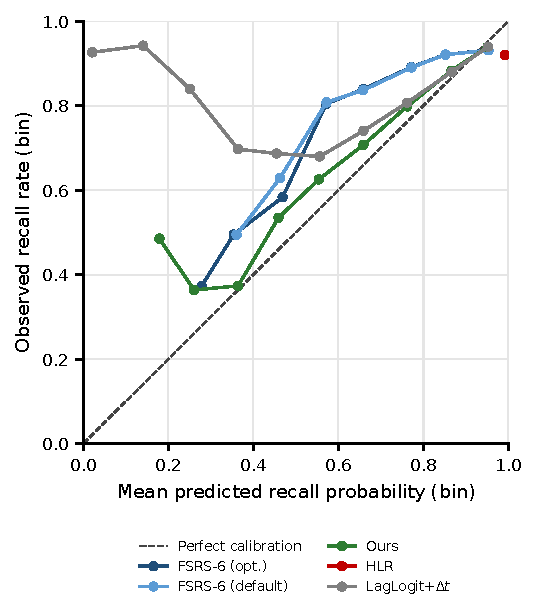
\includegraphics[width=12cm]{figures/data/fig_exp3_reliability.pdf}
  \caption[Experiment 3: reliability diagram]{Experiment 3: reliability diagram on the scored reviews. Each point is a
    bin of predicted probability with at least 20 reviews, plotted at its mean prediction and observed recall rate.
    HLR is a single point because all of its predictions fall in the top bin, so its other bins have fewer than 20
    reviews. The dashed diagonal is perfect calibration.}
  \label{fig:fig_exp3_reliability}
\end{figure}

The paired comparisons are in Figure~\ref{fig:fig_exp3_paired_forest}. Against FSRS-6 (optimised), the proposed model
has a lower log loss by $0.032$ (interval $[-0.033, -0.031]$), a lower Brier score by $0.006$, a higher AUC by
$0.087$ (interval $[+0.083, +0.091]$) and a lower ECE by $0.036$. All these intervals exclude zero. Against
LagLogit+$\Delta t$, the log-loss difference is $-0.023$ (interval $[-0.025, -0.021]$), and the AUC difference is
$+0.003$ (interval $[+0.001, +0.004]$). Both intervals exclude zero, but the AUC difference is very small, so
the interval excluding zero should not be read as a practical gap. 

\begin{figure}[htbp]
  \centering
  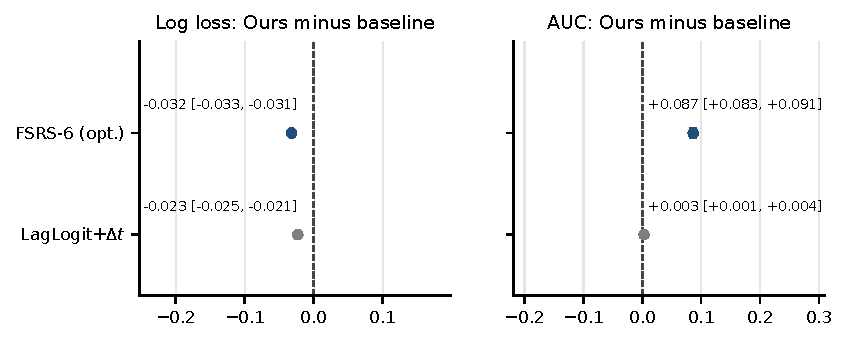
\includegraphics[width=\textwidth]{figures/data/fig_exp3_paired_forest.pdf}
  \caption[Experiment 3: paired differences]{Experiment 3: paired differences, the proposed model minus FSRS-6
    (optimised) (top row) and minus LagLogit+$\Delta t$ (bottom row), with 95\% user-clustered bootstrap intervals
    (1000 resamples). Left: log loss. Right: AUC. The dashed line marks zero. The LagLogit+$\Delta t$ row
    was computed separately from the predictions with the same bootstrap function. It is not in the run report.}
  \label{fig:fig_exp3_paired_forest}
\end{figure}

The per-user view is in Figure~\ref{fig:fig_exp3_user_wins}. Out of 41,223 users with a finite log loss for both
models, the proposed model has the lower per-user log loss for 30,511 users (74.0\%) against FSRS-6 (optimised).
LagLogit+$\Delta t$ does so for 29,525 users (71.6\%). HLR beats FSRS-6 (optimised) for 23,766 users (57.7\%).
Against LagLogit+$\Delta t$, the proposed model wins for only 17,721 users (43.0\%).

The first result is therefore a clear win on the aggregate metrics: on Duolingo, the proposed model has the lowest
log loss, the highest AUC and the lowest calibration error of the five models. Four caveats apply with equal weight.

\begin{enumerate}
  \item \textbf{FSRS-6 (optimised) is essentially the default model here.} It fell back to default weights for
    115,110 of 115,222 users, so the comparison with FSRS-6 is mainly a comparison with its default weights.
  \item \textbf{There are no grades.} FSRS-6 receives only Again and Good, and the proposed model receives the
    same binary outcome. The comparison is therefore not a test of the grade information that Experiment~2 favours.
  \item \textbf{The gain over LagLogit+$\Delta t$ comes mostly from the lighter half of users.} The proposed model beats LagLogit+$\Delta t$ for only 43.0\% of users (17,721 of 41,223). Table~\ref{tab:exp3-quartiles} splits users into quartiles by their number of scored reviews. The lighter half of users, Q1 and Q2, holds 12.8\% of the events and supplies 55.8\% of the total gain, although only 34--37\% of those users beat LagLogit+$\Delta t$. The heaviest quartile holds 65.7\% of the events, supplies 16.8\% of the gain, and gains only 0.006 per event. The median user is slightly worse with the proposed model, with a gain of $-0.0028$.
  \item \textbf{The chains did not converge.} The GPU run is a single chain with 100 kept draws, and its
    split $\hat R$ values are well above the gate. The Duolingo numbers are therefore provisional, as the Anki
    numbers are (Section~\ref{sec:results-mcmc}).
\end{enumerate}



\begin{figure}[htbp]
  \centering
  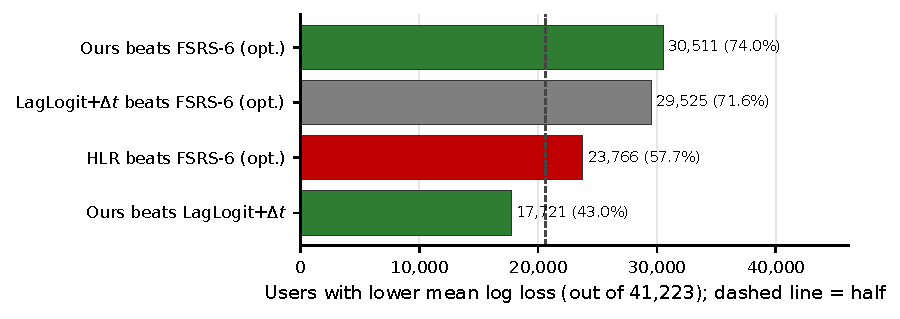
\includegraphics[width=\textwidth]{figures/data/fig_exp3_user_wins.pdf}
  \caption[Experiment 3: users with lower log loss]{Experiment 3: number of the 41,223 users with a finite log loss
    for both models for whom the first model has lower mean log loss than the second. The dashed line marks half
    of the users. The bottom bar is the only comparison in which the proposed model wins on fewer than half of the users.}
  \label{fig:fig_exp3_user_wins}
\end{figure}

\begin{table}[t]
  \centering
  \small
  \caption[Experiment 3: gain by user volume]{Experiment 3: users split into quartiles by number of scored reviews (41,223
    users). Gain is LagLogit log loss minus the proposed model's, per event. Events and share of events are descriptive.
    Bold marks the largest gain per event and the highest win share.}
  \label{tab:exp3-quartiles}
  \begin{tabular}{@{}lccc@{}}
    \toprule
    Quartile & Events (share) & Gain/event & Users won \& gain share \\
    \midrule
    Q1 (lightest) & 39,220 (3.3\%) & \textbf{0.136} & 34.2\% \& 19.7\% \\
    Q2 & 113,461 (9.5\%) & 0.086 & 37.3\% \& 36.1\% \\
    Q3 & 254,756 (21.4\%) & 0.029 & 49.1\% \& 27.4\% \\
    Q4 (heaviest) & 781,918 (65.7\%) & 0.006 & \textbf{51.3\%} \& 16.8\% \\
    \midrule
    Median user & \multicolumn{3}{c}{gain $-0.0028$} \\
    \bottomrule
  \end{tabular}
\end{table}

\section{Experiment 4: Improved Models}
\label{sec:results-exp4}

Experiments~2 and~3 left an open question. The proposed model won on Duolingo and lost on Anki, and its
chains did not converge, so it was unclear how much of the error was due to the memory model and how much to
the learner and the data. Experiment~4 adds three models that were built to answer it: the two MAP variants of the
hierarchy, v2 and v3, and a gradient-boosted tree model (GBDT) with no memory equation
(Section~\ref{sec:method-improved}). The title and the main model of this report remain the Bayesian model. Experiment~4
extends the study, and the results below show that a non-Bayesian predictor is the most accurate.

\subsection{Protocol}
\label{sec:results-exp4-protocol}

The protocol is that of Experiments~2 and~3: the same 100 Anki users and the same full Duolingo data, the same
temporal split, the same scored reviews (95,400 on Anki and 1,189,355 on Duolingo), the same metrics and the same
user-clustered paired bootstrap (1000 resamples, seed 0). The models were run again in one final run per dataset
(\texttt{full\_u100\_c1000\_final} and \texttt{duolingo\_final}). The rows for HLR, FSRS-6 and the proposed model (v1,
the MCMC model) are identical to those of Experiments~2 and~3, so the tables below repeat them. Model selection used
validation data only: the last 20\% of each user's training days, with all 100 users on Anki (74,092 scored
reviews) and a sample of 5,000 users on Duolingo (26,084 scored reviews). The selection rule was fixed before the runs. Among
the variants that were not significantly worse than FSRS-6 (optimised) on either dataset, it picked the lowest mean
validation log loss over the two datasets. Six stacked combinations were tried and none beat the GBDT alone, so the
GBDT alone is the final model.

\subsection{Overall results}
\label{sec:results-exp4-overall}

Tables~\ref{tab:exp4-anki} and~\ref{tab:exp4-duo} give the overall metrics. On both datasets the GBDT is the best
model on every metric. On Anki its log loss is 0.358, against 0.379 for FSRS-6 (optimised) and 0.422 for the proposed
model (v1). Its AUC on Anki is 0.805 against 0.777 for FSRS-6 (optimised). On Duolingo its log loss is 0.259, against
0.300 for FSRS-6 (optimised), 0.268 for the proposed model (v1) and 0.283 for v3, and its AUC is 0.697 against 0.656
for the proposed model (v1). Its calibration is very close to perfect on Duolingo (ECE 0.001, mean bias 0.000).
The MAP variants sit between the other models. On Anki, v2 and v3 have log loss 0.379 and 0.378, level with FSRS-6
(optimised). On Duolingo they improve on FSRS-6 (optimised) (0.289 and 0.283 against 0.300) but do not reach the proposed
model (v1) at 0.268. Figure~\ref{fig:fig_exp4_overall_bars} plots the log
losses of all models on both datasets.

\begin{table}[htbp]
  \centering
  \caption[Experiment 4: overall metrics on Anki]{Experiment 4: overall metrics on Anki, 95,400 scored reviews. Log loss, Brier, ECE,
    RMSE$_{\mathrm{bins}}$ and the absolute value of the mean bias are lower-is-better, and AUC is higher-is-better. Bold marks the best
    value in each column; for the mean bias, the best value is the one closest to zero, and a tie at three decimals is
    decided on the unrounded value. Ours (v1) is the MCMC model of Experiment~2.}
  \label{tab:exp4-anki}
  \begin{tabular}{@{}lcccccc@{}}
    \toprule
    Model & Log loss & Brier & AUC & ECE & RMSE$_{\mathrm{bins}}$ & Mean bias \\
    \midrule
    FSRS-6 (default) & 0.396 & 0.121 & 0.745 & 0.012 & 0.017 & $+0.011$ \\
    FSRS-6 (optimised) & 0.379 & 0.117 & 0.777 & 0.009 & 0.014 & $-0.002$ \\
    HLR & 0.680 & 0.170 & 0.555 & 0.146 & 0.176 & $+0.060$ \\
    Ours v1 (MCMC) & 0.422 & 0.131 & 0.692 & 0.025 & 0.032 & $+0.011$ \\
    Ours v2 (MAP) & 0.379 & 0.117 & 0.778 & 0.013 & 0.020 & $-0.009$ \\
    Ours v3 (MAP) & 0.378 & 0.117 & 0.779 & 0.010 & 0.018 & $-0.007$ \\
    GBDT & \textbf{0.358} & \textbf{0.111} & \textbf{0.805} & \textbf{0.005} & \textbf{0.010} & \textbf{$+0.002$} \\
    \bottomrule
  \end{tabular}
\end{table}

\begin{table}[htbp]
  \centering
  \caption[Experiment 4: overall metrics on Duolingo]{Experiment 4: overall metrics on full Duolingo, 1,189,355 scored reviews. Bold and
    the direction of each metric are as in Table~\ref{tab:exp4-anki}. Ours (v1) is the GPU port of the MCMC model of Experiment~3.}
  \label{tab:exp4-duo}
  \begin{tabular}{@{}lcccccc@{}}
    \toprule
    Model & Log loss & Brier & AUC & ECE & RMSE$_{\mathrm{bins}}$ & Mean bias \\
    \midrule
    FSRS-6 (default) & 0.302 & 0.078 & 0.566 & 0.051 & 0.070 & $-0.025$ \\
    FSRS-6 (optimised) & 0.300 & 0.078 & 0.570 & 0.050 & 0.070 & $-0.026$ \\
    HLR & 0.418 & 0.079 & 0.521 & 0.072 & 0.072 & $+0.072$ \\
    LagLogit+$\Delta t$ & 0.291 & 0.076 & 0.653 & 0.020 & 0.068 & $-0.001$ \\
    Ours v1 (MCMC) & 0.268 & 0.071 & 0.656 & 0.014 & 0.017 & $+0.004$ \\
    Ours v2 (MAP) & 0.289 & 0.075 & 0.609 & 0.035 & 0.048 & $-0.007$ \\
    Ours v3 (MAP) & 0.283 & 0.074 & 0.613 & 0.032 & 0.044 & $-0.010$ \\
    GBDT & \textbf{0.259} & \textbf{0.070} & \textbf{0.697} & \textbf{0.001} & \textbf{0.003} & \textbf{$+0.000$} \\
    \bottomrule
  \end{tabular}
\end{table}

\begin{figure}[htbp]
  \centering
  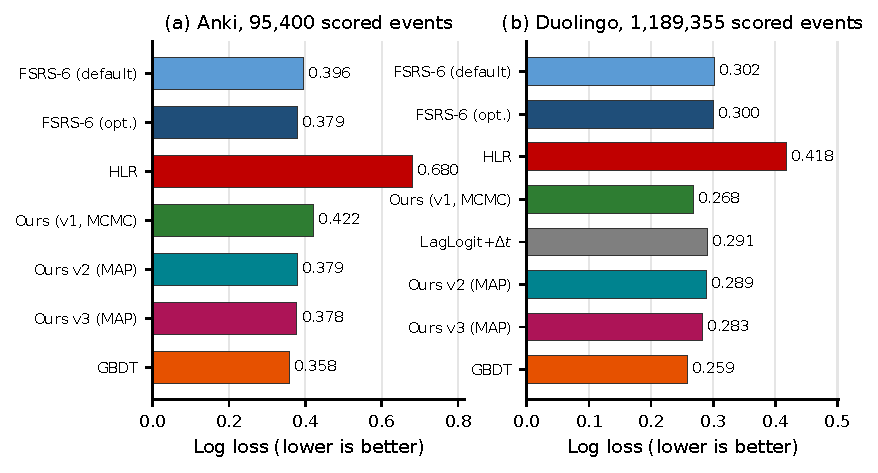
\includegraphics[width=\textwidth]{figures/data/fig_exp4_overall_bars.pdf}
  \caption[Experiment 4: overall log loss]{Experiment 4: overall log loss of every model on Anki (left, 95,400 scored reviews) and on
    full Duolingo (right, 1,189,355 scored reviews). Each bar starts at zero. The GBDT has the shortest bar on both datasets. LagLogit+$\Delta t$
    was not run on Anki.}
  \label{fig:fig_exp4_overall_bars}
\end{figure}

\subsection{Paired comparisons and user wins}
\label{sec:results-exp4-paired}

Table~\ref{tab:exp4-paired} gives the paired log-loss differences against FSRS-6 (optimised), with 95\% user-clustered
bootstrap intervals, and Figure~\ref{fig:fig_exp4_paired_forest} plots them. A negative difference favours the model. On Anki, v2 and v3 are not distinguishable from
FSRS-6 (optimised), because both intervals include zero. The GBDT is better by 0.021 in log loss, and its interval
excludes zero. Against the proposed model (v1) the GBDT is better on Anki by 0.064, with the interval $[-0.078, -0.052]$.
On Duolingo every difference in the table excludes zero, from $-0.011$ for v2 to $-0.041$ for the GBDT. The Duolingo intervals are narrow
because there are 41,223 users and 1,189,355 scored reviews. They describe sampling variation of the users and say nothing about the
leakage or selection issues of Section~\ref{sec:results-exp4-disclosures}.

\begin{table}[htbp]
  \centering
  \caption[Experiment 4: paired log-loss differences]{Experiment 4: paired log-loss difference, model minus FSRS-6 (optimised), with 95\% user-clustered bootstrap
    intervals (1000 resamples, seed 0). An asterisk marks an interval that excludes zero. Negative favours the model. The last row is the GBDT minus the proposed
    model (v1) on Anki.}
  \label{tab:exp4-paired}
  \begin{tabular}{@{}lcc@{}}
    \toprule
    Model & Anki & Duolingo \\
    \midrule
    Ours v1 (MCMC) & $+0.043$ [$+0.033$, $+0.055$]$^{*}$ & $-0.032$ [$-0.033$, $-0.031$]$^{*}$ \\
    Ours v2 (MAP) & $-0.000$ [$-0.003$, $+0.003$] & $-0.011$ [$-0.012$, $-0.010$]$^{*}$ \\
    Ours v3 (MAP) & $-0.001$ [$-0.004$, $+0.002$] & $-0.017$ [$-0.018$, $-0.016$]$^{*}$ \\
    GBDT & $-0.021$ [$-0.028$, $-0.014$]$^{*}$ & $-0.041$ [$-0.042$, $-0.041$]$^{*}$ \\
    \midrule
    GBDT minus Ours v1 & $-0.064$ [$-0.078$, $-0.052$]$^{*}$ & -- \\
    \bottomrule
  \end{tabular}
\end{table}

\begin{figure}[htbp]
  \centering
  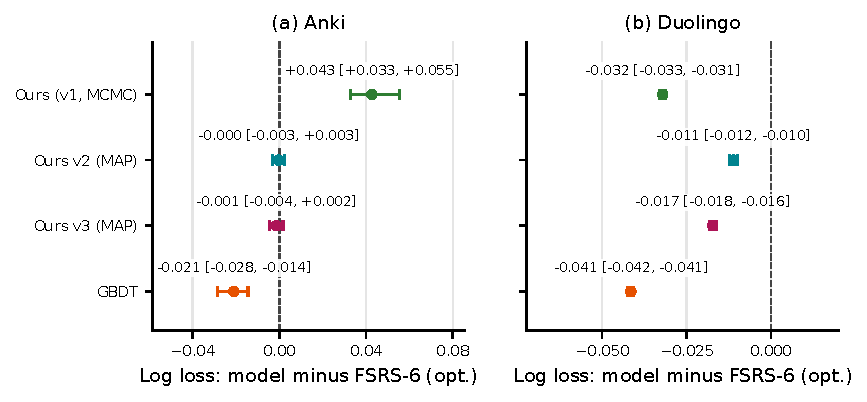
\includegraphics[width=\textwidth]{figures/data/fig_exp4_paired_forest.pdf}
  \caption[Experiment 4: paired differences]{Experiment 4: paired log-loss difference of the proposed model (v1), v2, v3 and the GBDT against
    FSRS-6 (optimised), with 95\% bootstrap intervals, on Anki (left) and Duolingo (right). The dashed line is zero; points to its
    left favour the model.}
  \label{fig:fig_exp4_paired_forest}
\end{figure}

Per-user results show the same order. Against FSRS-6 (optimised), the number of Anki users (of 100) on whom the model has lower log loss is 56 for v2, 58 for v3 and 82 for the
GBDT, and the GBDT beats the proposed model (v1) on 94 of the 100 users. On Duolingo (41,223 users) the shares of users won against FSRS-6
(optimised) are 70.4\% for v2, 71.5\% for v3 and 78.0\% for the GBDT.

\subsection{Overfitting checks}
\label{sec:results-exp4-overfit}

A tree model with many features can overfit, so three checks were made on data that the model did not see
(Figure~\ref{fig:fig_exp4_overfit}). First, the GBDT's validation log loss on Anki is 0.3614 and its test log loss is 0.3584, and on Duolingo the
validation value (5,000-user dev sample) is 0.2578 and the test value (all users) is 0.2588. The test values are close to the validation values, and neither
test value is much worse. Second, on Anki the GBDT's log loss on its own training rows (341,739 rows) is 0.3467, against 0.3584 on the test rows, a gap of
0.012. Third, among the scored Duolingo users, 2,004 have no training rows (15,918 scored reviews; 64,254 users overall have none), and on them the GBDT has log loss 0.2329, against 0.2604 for v3, 0.2647 for the proposed model (v1) and 0.2748 for
FSRS-6 (optimised) on Duolingo. The GBDT's lead is therefore largest on users it has never seen. A leakage audit also found one real leak, which is reported next. These
checks reduce the worry about overfitting on these data. They do not remove the selection effects of Section~\ref{sec:results-exp4-disclosures}.

\begin{figure}[htbp]
  \centering
  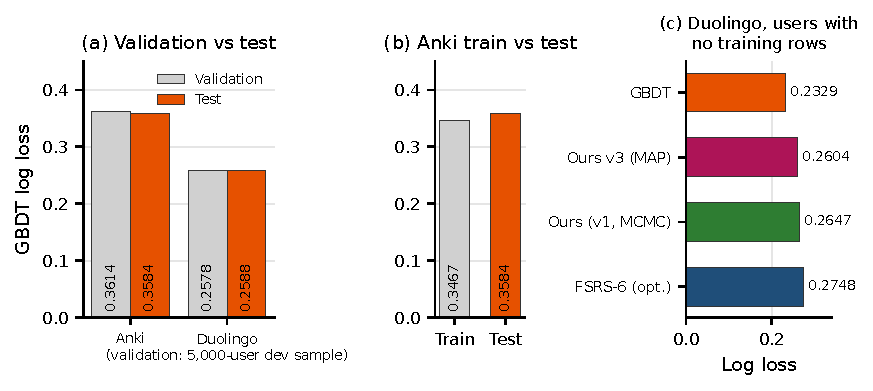
\includegraphics[width=\textwidth]{figures/data/fig_exp4_overfit.pdf}
  \caption[Experiment 4: overfitting checks]{Experiment 4: overfitting checks of the GBDT. (a) Validation against test log loss on both datasets; the Duolingo
    validation value uses the 5,000-user dev sample. (b) Anki log loss on the training rows against the test rows. (c) Duolingo log loss on the 2,004 scored users with no training rows (15,918 scored reviews).}
  \label{fig:fig_exp4_overfit}
\end{figure}

\subsection{A same-session leak and its fix}
\label{sec:results-leak}

The first version of the GBDT had a leak that the design of Chapter~\ref{ch:dataset} did not anticipate. Duolingo logs one practice session at a single
timestamp, so several reviews of different cards share the same time. A running user statistic such as the user's recall so far then
included the outcomes of other reviews of the same session, some of which come after the scored review within the session, so a feature could see
outcomes that were not yet known. The check was a validation run: the log loss on the 5,000-user dev sample was 0.2473 with the leak, a value that was too good
to be true, and 0.2578 once rows with the same timestamp were grouped so that a review sees none of its own session. The grouped value is the valid one, and all
GBDT numbers in this report use it. The leaky sweep of 38 variants was discarded, and the selection was repeated on 16 variants per dataset after the fix. This is the pitfall that the same-timestamp rule of
Section~\ref{sec:method-gbdt} prevents.

\subsection{Disclosures}
\label{sec:results-exp4-disclosures}

The following points limit how far the Experiment~4 results can be trusted, and each is stated as it happened.

\begin{enumerate}[label=(\alph*)]
  \item The test set was looked at twice. The v2 model was scored on it in an earlier phase, and v3 and the GBDT were scored on it later, with the GBDT configuration frozen before that run.
  \item The selection rule for v2 was revised after its validation intervals were seen, so the rule for v2 is not fully pre-specified.
  \item Many variants were tried: 9 for v2, 23 for v3, 38 for the GBDT in the leaky sweep and then 16 per dataset after the fix, and 6 stackers. The reported models are the winners
    of searches, so their validation values are optimistic. The test values are less affected by the search, but see item (a).
  \item The same-session leak of Section~\ref{sec:results-leak} was found and fixed by grouping rows with the same timestamp. The invalid value 0.2473 was replaced by the valid value 0.2578.
  \item The Duolingo lexeme recall rate pools the training rows of other users that fall later in calendar time. The effect was about 0.001 in log loss. This is an accepted limitation.
  \item The models v2 and v3 are fitted by MAP, so they give point estimates, with no posterior and no convergence diagnostics, and they are not Bayesian in their inference.
  \item The learned rate $\lambda$ of the proposed model (v1) did not converge on Duolingo, as reported in Section~\ref{sec:results-mcmc}.
  \item On Duolingo, FSRS-6 (optimised) is practically the default model, because it keeps the default weights for almost all users (115,110 of 115,222), so the gain over FSRS-6 on Duolingo is a gain over the default weights.
  \item The GBDT does not use the history counters supplied with the Duolingo logs or the state column of the Anki logs.
\end{enumerate}

The GBDT also has limits of its own. It is a pure predictor, with no stability or difficulty state that a scheduler could use. The results come from one seed and one split, on 100 Anki users, and no scheduling simulation was run.
A GRU model and an ensemble of v1 and v2 were not completed. The GBDT was later run inside the larger \texttt{srs-benchmark} protocol (Section~\ref{sec:results-exp5-srsb}).

\subsection{Where the gain comes from, and related work}
\label{sec:results-exp4-source}

The gain comes mostly from running statistics of the user's own performance and from training on all non-first reviews, and not from a memory model. Dropping the user feature group raises the GBDT's validation log loss on Anki from 0.363 to 0.377. This means that the GBDT's
advantage is a cross-card signal of the learner's ability, which a model that treats each card in isolation does not use.

This signal is not new. DASH \cite{lindsey2014improving} and DAS3H \cite{choffin2019das3h} use past practice across items, and
the winning entry of the Second Language Acquisition Modeling task combined LightGBM with a recurrent network \cite{settles2018slam,osika2018slam}. The \texttt{srs-benchmark} of about ten thousand Anki users \cite{srsbenchmark}
has no tree model among its published models. Its best published model, RWKV-Instant, also uses history across cards. The benchmark's own published results on the full collection give it a log loss of 0.277 against 0.346 for FSRS-6 \cite{srsbenchmark}. These figures are cited for context only: they come from a different sample and are not comparable with Table~\ref{tab:exp4-anki}. Our comparison on 1,000 of the benchmark's users, under its protocol, is in Section~\ref{sec:results-exp5-srsb}. What is specific here is the use of FSRS-state features in the trees, a leakage-audited protocol on two datasets, and the comparison with a Bayesian model.

\subsection{Cost}
\label{sec:results-exp4-cost}

Table~\ref{tab:exp4-cost} gives the fit and predict times of the three new models. They are small next to the sampler of Section~\ref{sec:results-cost}.

\begin{table}[htbp]
  \centering
  \caption[Experiment 4: fit and predict times]{Experiment 4: fit and predict wall-clock time in seconds.}
  \label{tab:exp4-cost}
  \begin{tabular}{@{}lcccc@{}}
    \toprule
    & \multicolumn{2}{c}{Anki} & \multicolumn{2}{c}{Duolingo} \\
    \cmidrule(lr){2-3}\cmidrule(lr){4-5}
    Model & Fit & Predict & Fit & Predict \\
    \midrule
    Ours v2 (MAP) & 25.7 & 3.1 & 489 & 26 \\
    Ours v3 (MAP) & 23.7 & 3.2 & 756 & 28 \\
    GBDT & 26.8 & 2.1 & 265 & 90 \\
    \bottomrule
  \end{tabular}
\end{table}

\section{Experiment 5: Constant Floors, Robustness and srs-benchmark}
\label{sec:results-exp5}

Experiments~2 to~4 compare models with each other. Experiment~5 asks three further questions. How much of
each model's log loss is no more than the base rate of recall? Do the Anki results of Experiment~4 hold on
other samples of users? And do they hold on the published srs-benchmark protocol, which uses a different and
larger set of users? The Duolingo and main Anki numbers are taken from the final result files of the two benchmarks,
and the seed and srs-benchmark numbers from the runs described below.

\subsection{Constant floors}
\label{sec:results-exp5-floors}

A constant floor is a predictor with no memory model. It gives every review the same predicted recall
probability, so it measures what a model gains from the review history alone. Three floors were fitted on the
training rows of each dataset and scored on the same test reviews as the other models. The global floor predicts
the training recall rate for every user. The per-user floor predicts each user's own training recall rate. The
smoothed per-user floor pulls each user's rate toward the global rate with a pseudo-count of $m = 10$, so that a
user with few training reviews is not predicted from a noisy rate. Table~\ref{tab:exp5-floors} gives their log
losses.

\begin{table}[htbp]
  \centering
  \caption[Experiment 5: constant floors]{Experiment 5: log loss of the three constant floors on each dataset, on the same scored
    reviews as Experiments~2 to~4 (95,400 on Anki and 1,189,355 on Duolingo). Lower is better. Bold marks the lower value in each column.}
  \label{tab:exp5-floors}
  \begin{tabular}{@{}lcc@{}}
    \toprule
    Floor & Anki & Duolingo \\
    \midrule
    Constant (global) & 0.4544 & 0.2792 \\
    Constant (per user) & 0.4308 & 0.3725 \\
    Constant (per user, smoothed, $m = 10$) & \textbf{0.4307} & \textbf{0.2723} \\
    \bottomrule
  \end{tabular}
\end{table}

On Duolingo the smoothed per-user floor, at 0.2723, beats FSRS-6 (optimised) at 0.3003, FSRS-6 (default) at 0.3018, HLR
at 0.4181, LagLogit+$\Delta t$ at 0.2910, Ours v2 at 0.2892 and Ours v3 at 0.2830. Only two models beat it: the GBDT, at
0.2588, and the proposed model (v1), at 0.2682. The margin of v1 is small, but its interval excludes zero: v1 minus the
smoothed floor is $-0.0040$, with a 95\% user-clustered bootstrap interval of $[-0.0045, -0.0035]$. FSRS-6 (optimised)
minus the same floor is $+0.0280$, with interval $[+0.0271, +0.0289]$. On Anki the floors are much higher, and every model
except HLR beats all three of them. The smoothed floor is 0.4307, FSRS-6 (optimised) is 0.3794 and v1 is 0.4221. FSRS-6 (optimised) minus the smoothed floor is $-0.0513$, with interval $[-0.0669, -0.0391]$, and v1 minus the floor is
$-0.0086$, with interval $[-0.0140, -0.0040]$.
HLR is worse than the global constant on both datasets: 0.6805 against 0.4544 on Anki, and 0.4181 against 0.2792 on
Duolingo. On these data, HLR as fitted here carries less information than the base rate.

Figure~\ref{fig:fig_exp5_floors} plots the log loss of every model on both datasets, with the three floors as dashed
reference lines. Bars that stand below a line beat that floor.

\begin{figure}[htbp]
  \centering
  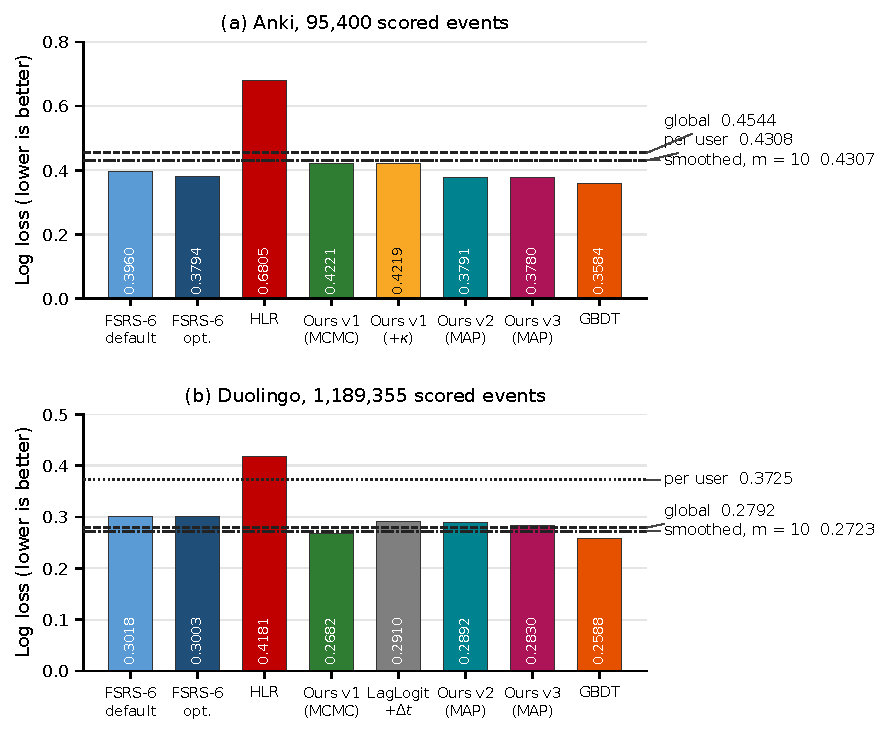
\includegraphics[width=\textwidth]{figures/data/fig_exp5_floors.pdf}
  \caption[Experiment 5: log loss against the constant floors]{Experiment 5: overall log loss of every model on Anki (top, 95,400 scored
    reviews) and on Duolingo (bottom, 1,189,355 scored reviews). The three dashed lines are the constant floors: global (dashed), per user
    (dotted) and per user smoothed with $m = 10$ (dash-dot). Ours v1 (+$\kappa$) is shown on Anki only, and LagLogit+$\Delta t$ on Duolingo only.}
  \label{fig:fig_exp5_floors}
\end{figure}

\subsection{Robustness over three Anki samples}
\label{sec:results-exp5-seeds}

The Anki results of Experiments~2 and~4 come from one sample of 100 users. Two further independent samples of 100
users were drawn with seeds 1 and 2. Each model except v1 was run on each sample with frozen settings. Seed 0 is the sample of the main Anki benchmark. The proposed model (v1) was not re-run on seeds 1 and 2, so it
is left out of Table~\ref{tab:exp5-seeds}. The smoothed per-user floor is not in the seed files either.

\begin{table}[htbp]
  \centering
  \caption[Experiment 5: log loss over three Anki samples]{Experiment 5: overall log loss on three independent samples of 100 Anki users, with the
    mean and the range (maximum minus minimum) over the three seeds. Lower is better. Bold marks the lowest value in each column.}
  \label{tab:exp5-seeds}
  \begin{tabular}{@{}lccccc@{}}
    \toprule
    Model & Seed 0 & Seed 1 & Seed 2 & Mean & Range \\
    \midrule
    Constant (global) & 0.4544 & 0.3930 & 0.4329 & 0.4268 & 0.0613 \\
    Constant (per user) & 0.4308 & 0.3613 & 0.4063 & 0.3995 & 0.0695 \\
    FSRS-6 (default) & 0.3960 & 0.3246 & 0.3641 & 0.3616 & 0.0714 \\
    FSRS-6 (optimised) & 0.3794 & 0.3142 & 0.3521 & 0.3486 & 0.0651 \\
    HLR & 0.6805 & 0.5553 & 0.5953 & 0.6104 & 0.1252 \\
    Ours v3 (MAP) & 0.3780 & 0.3081 & 0.3510 & 0.3457 & 0.0699 \\
    GBDT & \textbf{0.3584} & \textbf{0.2916} & \textbf{0.3311} & \textbf{0.3271} & 0.0668 \\
    \bottomrule
  \end{tabular}
\end{table}

The seven rows of Table~\ref{tab:exp5-seeds} are in the same order on all three samples. The GBDT has the lowest log loss on
each sample, and HLR the highest. Table~\ref{tab:exp5-seed-diff} gives the GBDT's paired difference from FSRS-6 (optimised) on each sample,
with 95\% user-clustered bootstrap intervals (1000 resamples). Each interval excludes zero. The last row is the mean of the
three differences, which is a summary of three estimates and has no interval of its own.

\begin{table}[htbp]
  \centering
  \caption[Experiment 5: GBDT minus FSRS-6 over three samples]{Experiment 5: paired log-loss difference, GBDT minus FSRS-6 (optimised), per
    Anki sample, with 95\% user-clustered bootstrap intervals. An asterisk marks an interval that excludes zero. Negative favours the GBDT.}
  \label{tab:exp5-seed-diff}
  \begin{tabular}{@{}lcc@{}}
    \toprule
    Sample & Difference & 95\% interval \\
    \midrule
    Seed 0 (main benchmark) & $-0.0210$ & $[-0.0284, -0.0144]^{*}$ \\
    Seed 1 & $-0.0226$ & $[-0.0371, -0.0137]^{*}$ \\
    Seed 2 & $-0.0210$ & $[-0.0325, -0.0119]^{*}$ \\
    \midrule
    Mean of the three & $-0.0215$ & not reported \\
    \bottomrule
  \end{tabular}
\end{table}

FSRS-6 (optimised) fell back to its default weights for 1 of the 100 users on seed 0, for 4 users on seed 1 and for 6 users on
seed 2. These fallbacks are few on Anki. On Duolingo the fallback covers almost every user (Section~\ref{sec:results-exp4-disclosures}),
and the seed results say nothing about that case.

\subsection{The srs-benchmark comparison}
\label{sec:results-exp5-srsb}

The srs-benchmark project \cite{srsbenchmark} publishes results for recall models on the full \texttt{anki-revlogs-10k}
collection of 9,999 users, with its own test folds. To put the GBDT against those results, the benchmark's protocol was
followed. A pooled GBDT, one LightGBM model fitted on the rows of other users with past-only features, was trained on
users 9001 to 9500 (450 users for fitting and 50 held out) and evaluated on users 1 to 1000 with the benchmark's own test
folds (\texttt{--algo FSRS-6 --short}, five time-series folds). The training users and the evaluation users are disjoint by
id. The fit used 17,060,060 rows. Each evaluated user has the published test-row count, so all 1000 users match the size of
the benchmark's own runs. The other models' values are those of the srs-benchmark result files for the same 1000 users, so
every row of Table~\ref{tab:exp5-srsb} is computed on one set of users. These numbers are not comparable with the 100-user
Anki sample of Table~\ref{tab:exp4-anki}.

Table~\ref{tab:exp5-srsb} gives log loss and AUC for every model in the comparison, unweighted (the mean over users) and
weighted by each user's test size. Table~\ref{tab:exp5-srsb-paired} gives the GBDT's paired log-loss differences, weighted,
with 99\% user-clustered bootstrap intervals.

\begin{table}[htbp]
  \centering
  \caption[Experiment 5: srs-benchmark comparison]{Experiment 5: log loss and AUC on the srs-benchmark's 1000 evaluation users, for the
    pooled GBDT and the eleven models listed by the benchmark. ``Unweighted'' is the mean over users and ``weighted'' is
    weighted by each user's test-row count. Log loss is lower-is-better and AUC is higher-is-better. Bold marks the best value
    in each column.}
  \label{tab:exp5-srsb}
  \begin{tabular}{@{}lcccc@{}}
    \toprule
    & \multicolumn{2}{c}{Log loss} & \multicolumn{2}{c}{AUC} \\
    \cmidrule(lr){2-3}\cmidrule(lr){4-5}
    Model & Unweighted & Weighted & Unweighted & Weighted \\
    \midrule
    RWKV-Instant & \textbf{0.2860} & \textbf{0.2828} & \textbf{0.8319} & \textbf{0.8265} \\
    GBDT (pooled, ours) & 0.3211 & 0.3148 & 0.7780 & 0.7666 \\
    RWKV-Curve & 0.3302 & 0.3143 & 0.7665 & 0.7712 \\
    GRU & 0.3441 & 0.3271 & 0.7298 & 0.7337 \\
    LSTM & 0.3445 & 0.3271 & 0.7311 & 0.7358 \\
    MOVING-AVG & 0.3462 & 0.3372 & 0.7007 & 0.6968 \\
    FSRS-7 (recency) & 0.3485 & 0.3308 & 0.7208 & 0.7243 \\
    Logistic Regression & 0.3502 & 0.3341 & 0.7090 & 0.7104 \\
    FSRS-6 & 0.3580 & 0.3383 & 0.6994 & 0.7061 \\
    DASH & 0.3792 & 0.3571 & 0.6316 & 0.6407 \\
    AVG & 0.4055 & 0.3802 & 0.5007 & 0.5053 \\
    HLR & 0.4877 & 0.4479 & 0.6352 & 0.6299 \\
    \bottomrule
  \end{tabular}
\end{table}

\begin{table}[htbp]
  \centering
  \caption[Experiment 5: paired differences on srs-benchmark]{Experiment 5: GBDT minus each baseline, size-weighted log loss, with 99\% user-clustered
    bootstrap intervals (1000 resamples, same users). An asterisk marks an interval that excludes zero. Negative favours the GBDT. The comparison output
    gives paired differences for these six models only.}
  \label{tab:exp5-srsb-paired}
  \begin{tabular}{@{}lcc@{}}
    \toprule
    Baseline & Difference & 99\% interval \\
    \midrule
    FSRS-6 & $-0.0235$ & $[-0.0286, -0.0183]^{*}$ \\
    RWKV-Instant & $+0.0320$ & $[+0.0287, +0.0358]^{*}$ \\
    RWKV-Curve & $+0.0006$ & $[-0.0044, +0.0055]$ \\
    GRU & $-0.0123$ & $[-0.0174, -0.0067]^{*}$ \\
    AVG & $-0.0654$ & $[-0.0730, -0.0587]^{*}$ \\
    MOVING-AVG & $-0.0224$ & $[-0.0255, -0.0196]^{*}$ \\
    \bottomrule
  \end{tabular}
\end{table}

On the unweighted measure the pooled GBDT, at 0.3211, is better than FSRS-6 (0.3580), the GRU (0.3441) and the other
baselines in Table~\ref{tab:exp5-srsb}, and it is behind RWKV-Instant (0.2860). On the weighted measure the GBDT (0.3148)
is level with RWKV-Curve (0.3143): the difference is $+0.0006$ and its interval includes zero. On the same measure the GBDT is behind RWKV-Instant (0.2828), which is the best weighted log loss in Table~\ref{tab:exp5-srsb}. Against FSRS-6 the weighted
difference is $-0.0235$, with the interval $[-0.0286, -0.0183]$, which excludes zero.

The GBDT number is therefore a lower bound on what the model can do under this protocol. Boosting reached the cap of 2000
rounds at its best iteration, so early stopping did not trigger, and a larger cap was not tried.

\subsection{The leakage pitfall, again}
\label{sec:results-exp5-leak}

The same-timestamp pitfall of Section~\ref{sec:results-leak} is the one audit finding that Experiment~5 repeats. Duolingo logs one practice
session at a single timestamp, so a running feature can see outcomes that come after the scored review. On the 5,000-user dev sample the
GBDT scored 0.2473 with that leak and 0.2578 once same-timestamp rows were grouped. The Duolingo GBDT in this section and in
Figure~\ref{fig:fig_exp5_floors} is the grouped version, and the leaky value should not be read as a result. The srs-benchmark run
uses past-only features.

\section{Cross-Dataset Comparison}
\label{sec:results-cross}

Table~\ref{tab:cross} places the overall log losses from the two benchmarks side by side. Figure~\ref{fig:fig_cross_dataset}
shows the same values. Among the models of Experiments~2 and~3 (four on Anki, five on Duolingo), FSRS-6 (optimised) is the best on Anki and the proposed model is third, and on Duolingo the
order reverses: the proposed model is best and FSRS-6 (optimised) is third. HLR is last on both datasets. The three models of Experiment~4 (Section~\ref{sec:results-exp4}) are added to the table.
The GBDT has the lowest log loss on both datasets, so with all eight models the ranking at the top does not reverse, although the order of FSRS-6 and the proposed model still does. LagLogit+$\Delta t$
was not run on Anki, so it has no Experiment~2 value.

\begin{table}[htbp]
  \centering
  \caption[Overall log loss, Anki and Duolingo]{Overall log loss on the two benchmarks. Bold marks the lowest value in
    each column. The Anki values are from Experiments~2 and~4 and the Duolingo values from Experiments~3 and~4. LagLogit+$\Delta t$
    was not run on Anki.}
  \label{tab:cross}
  \begin{tabular}{@{}lcc@{}}
    \toprule
    Model & Anki & Duolingo \\
    \midrule
    FSRS-6 (optimised) & 0.379 & 0.300 \\
    FSRS-6 (default) & 0.396 & 0.302 \\
    HLR & 0.680 & 0.418 \\
    LagLogit+$\Delta t$ & -- & 0.291 \\
    Ours v1 (MCMC) & 0.422 & 0.268 \\
    Ours v2 (MAP) & 0.379 & 0.289 \\
    Ours v3 (MAP) & 0.378 & 0.283 \\
    GBDT & \textbf{0.358} & \textbf{0.259} \\
    \bottomrule
  \end{tabular}
\end{table}

\begin{figure}[htbp]
  \centering
  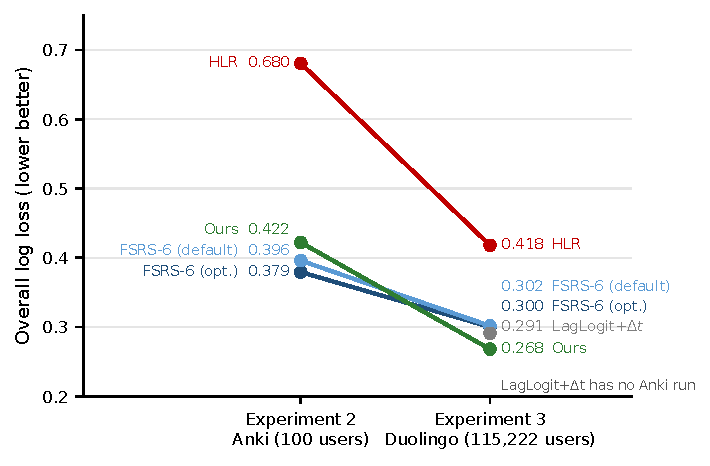
\includegraphics[width=12cm]{figures/data/fig_cross_dataset.pdf}
  \caption[Overall log loss across datasets]{Overall log loss per model on the Anki benchmark (left) and on Duolingo
    (right). Lines connect each model's two values; LagLogit+$\Delta t$ has only the Duolingo value. The order of
    FSRS-6 (optimised) and the proposed model (Experiments~2 and~3) reverses between the two datasets. The GBDT of Experiment~4 is not in this figure; see Figure~\ref{fig:fig_exp4_overall_bars}.}
  \label{fig:fig_cross_dataset}
\end{figure}

Several differences between the two benchmarks could account for the reversal. We did not test any of them, so they are
hypotheses for future work and not findings.

\begin{itemize}
  \item \textbf{Grades.} On Anki, FSRS-6 uses all four grades and the proposed model uses a binary outcome. The grade
    information is a candidate reason that FSRS-6 does better there. On Duolingo neither model has grades, so the
    advantage that grades could give is absent.
  \item \textbf{Per-user optimisation.} On Anki, FSRS-6 (optimised) fits its weights per user, and that fit is the
    best FSRS result. On Duolingo the fit falls back to defaults for almost all users, so the advantage of per-user
    fitting is absent.
  \item \textbf{Gap range.} Anki scored reviews reach 61 days and longer, where the proposed model over-predicts
    (Section~\ref{sec:results-exp2}). Duolingo scored reviews stop at 4--14 days.
  \item \textbf{Data size and sampler.} Duolingo has 115,222 users and 6,468,512 training events, against 100
    users and 606,364 training events on Anki. The Duolingo run also used the GPU port with fewer kept draws. A larger
    dataset may give the sampler more information, and the port may differ in its numerical behaviour. We cannot separate
    these effects with the runs we have.
\end{itemize}

The ranking of the proposed model and FSRS-6 therefore depends on the dataset, and this report does not claim that the proposed model is better than FSRS-6 in general. The GBDT, which uses none of these ingredients, is best among the models in this report on both datasets.

Experiment~5 (Section~\ref{sec:results-exp5-floors}) adds a reference point for each benchmark. On Duolingo, a per-user constant
that uses no memory model, smoothed toward the global rate, beats FSRS-6 (optimised) by $0.0280$, and the proposed model is only
$0.0040$ better than that constant. The Duolingo comparison above is therefore made against a demanding floor. On Anki the floors are
much higher, with the smoothed per-user constant at 0.4307, so FSRS-6 (optimised) and the MAP variants are well ahead of them. The
srs-benchmark sample of Section~\ref{sec:results-exp5-srsb} is a third collection, and its numbers do not enter Table~\ref{tab:cross}.

\section{MCMC Diagnostics}
\label{sec:results-mcmc}

The sampler's convergence was checked with the split $\hat R$ and the effective sample size (ESS). The gate used in
this report requires $\hat R < 1.01$ and an ESS of at least 400 for every scalar. Table~\ref{tab:mcmc} gives the values
for the three runs that were diagnosed. Experiment~2 has 250 kept draws per chain and Experiment~3 has 100. Both
Experiment~2 variants are single chains. No scalar in any of the three runs meets the ESS gate, and no run meets the
$\hat R$ gate for every scalar.

\begin{table}[htbp]
  \centering
  \caption[MCMC diagnostics]{Split $\hat R$ and effective sample size (ESS) per parameter, for three single-chain
    runs. A dash means the value is not reported. Bold marks the best value in each column: the highest ESS and the
    lowest $\hat R$.}
  \label{tab:mcmc}
  \begin{tabular}{@{}lcccccc@{}}
    \toprule
    & \multicolumn{2}{c}{Exp.\ 2, Ours} & \multicolumn{2}{c}{Exp.\ 2, Ours (+$\kappa$)} & \multicolumn{2}{c}{Exp.\ 3, Ours} \\
    \cmidrule(lr){2-3}\cmidrule(lr){4-5}\cmidrule(lr){6-7}
    Parameter & ESS & $\hat R$ & ESS & $\hat R$ & ESS & $\hat R$ \\
    \midrule
    $\lambda$ & 3.0 & 2.44 & 3.0 & 2.38 & 3 & 2.48 \\
    $\sigma^2$ & 3.3 & 2.07 & 9.3 & \textbf{1.16} & -- & 2.45 \\
    $b_0$ & 3.9 & 1.85 & 4.4 & 1.28 & -- & 1.77 \\
    $g_0$ & 80.6 & \textbf{1.00} & 234 & -- & 10 & -- \\
    $\tau^2_\alpha$ & \textbf{250} & \textbf{1.00} & \textbf{250} & -- & \textbf{20} & \textbf{1.01} \\
    $\tau^2_\beta$ & 4.8 & 1.88 & 9.0 & 1.26 & -- & 2.15 \\
    $\tau^2_\gamma$ & 143 & 1.06 & 202 & -- & -- & 2.64 \\
    $\kappa$ & -- & -- & 3.5 & 1.94 & -- & -- \\
    \bottomrule
  \end{tabular}
\end{table}

The learned rate $\lambda$ has the lowest ESS in every run, and in both Experiment~2 variants it also has the largest $\hat R$. Its ESS is 3 in both variants and in the Duolingo run, and its $\hat R$ is above 2.3 in all three. In Experiment~3 the user-slope variance $\tau^2_\gamma$ has the largest $\hat R$, at 2.64. The learned rate $\lambda$ is therefore
not estimated reliably by these chains. Figure~\ref{fig:fig_mcmc_ess_rhat} shows the ESS and $\hat R$ values for the two
Experiment~2 variants, on a logarithmic ESS scale. Every ESS bar is below the gate of 400, and most $\hat R$ values are
above the gate of 1.01. In the first Experiment~2 variant, $\tau^2_\alpha$ mixes best (ESS 250, $\hat R$ 1.00), and $\lambda$, $\sigma^2$ and $b_0$ have the lowest ESS (3.0, 3.3 and 3.9).

\begin{figure}[htbp]
  \centering
  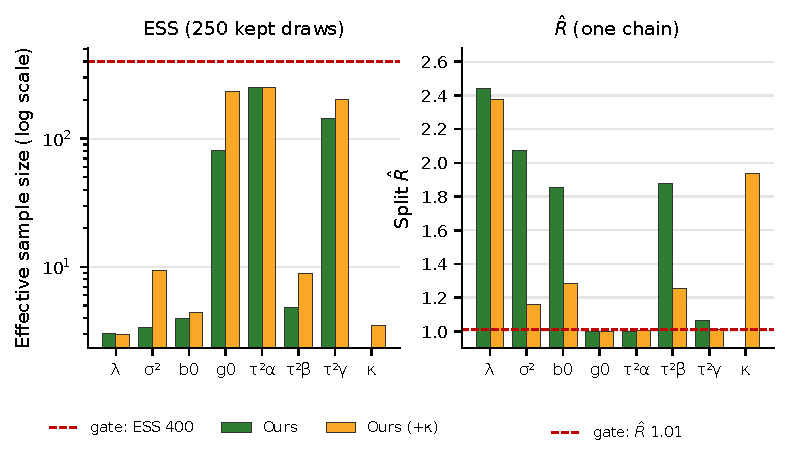
\includegraphics[width=\textwidth]{figures/data/fig_mcmc_ess_rhat.pdf}
  \caption[MCMC diagnostics, Experiment 2]{Experiment 2: effective sample size (left, logarithmic scale) and split
    $\hat R$ (right) for each parameter, for the two variants of the proposed model. Dashed lines mark the gates, ESS 400 and $\hat R$ 1.01.
    Every ESS value is below the gate, and most $\hat R$ values are above it.}
  \label{fig:fig_mcmc_ess_rhat}
\end{figure}

The fitted $\kappa$ in the proposed model's $+\kappa$ variant is $-0.160$, with an interval of $[-0.211, -0.076]$. This interval
excludes zero, but its chain did not converge. The sign and size of $\kappa$ are therefore not interpreted in this
report. A longer Experiment~2 run of 8000 sweeps was also started. That run was stopped at sweep 1400 of 8000 when the machine shut down. Figure~\ref{fig:fig_long_run_lambda}
shows the trace of $\lambda$ in the logged sweeps. The value rose from 0.34 to 1.70 and was still drifting upward when
the run stopped. It had not yet reached the benchmark posterior mean of 1.871 when the run stopped. The run gives no result, and it is reported
only as evidence that the chain had not settled.

\begin{figure}[htbp]
  \centering
  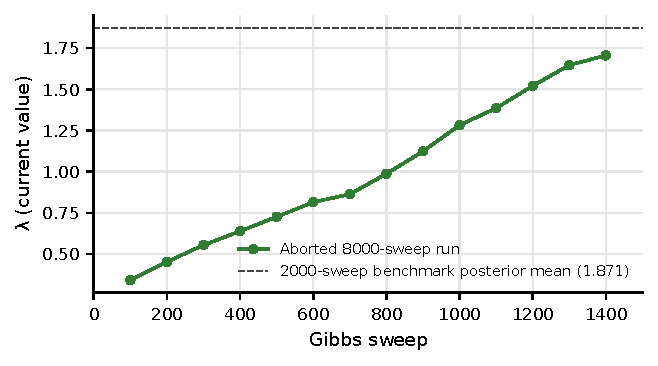
\includegraphics[width=\textwidth]{figures/data/fig_long_run_lambda.pdf}
  \caption[Aborted long run: trace of $\lambda$]{Trace of $\lambda$ in the aborted 8000-sweep Experiment~2 run, over the
    sweeps that were logged before the run stopped at sweep 1400. The dashed line is the posterior mean of the 2000-sweep
    benchmark run. The trace is still trending upward at the last logged sweep.}
  \label{fig:fig_long_run_lambda}
\end{figure}

The lack of convergence has a structural cause. Two identifiability problems follow from the model, and they are
not specific to the sampler. The first is a ridge between the rate $\lambda$ and the diffusion variance $\sigma^2$. Write
$\varphi = e^{-\lambda \Delta t}$ and let $q$ be the transition variance. When the gap is long, $\lambda \Delta t$ is large
and the transition depends on $\lambda$ and $\sigma^2$ only through their ratio,
\begin{equation}\label{eq:ridge-large}
  \varphi \to 0, \qquad q = \frac{\sigma^2\bigl(1-e^{-2\lambda\Delta t}\bigr)}{2\lambda} \to \frac{\sigma^2}{2\lambda}.
\end{equation}
Only $\sigma^2/\lambda$ is informed, so $\lambda$ and $\sigma^2$ can move along a ridge. When the gap is short, the
approximations change,
\begin{equation}\label{eq:ridge-small}
  \varphi \approx 1-\lambda\Delta t, \qquad q \approx \sigma^2 \Delta t,
\end{equation}
and the drift term $(1-\varphi)\mu$ is close to zero. The data then carry little information about $\lambda$ at all. Binary outcomes are coarse, which makes both effects harder to separate.

The second problem is a rank deficiency in the mean. The design matrices of the mean have 37 columns, but their rank is 33.
The four exact null directions are nested additive shifts of $b_0$, $\alpha_u$ and $\beta_i$, which leave the likelihood
unchanged. The population-level combination of the effects mixes better than $b_0$ alone. Reparameterising the mean is listed as future work in Chapter~\ref{ch:conclusion}.

\section{Task 3 Sampler Study}
\label{sec:results-task3}

The Task~3 study tested the sampler on synthetic data with known parameters, and then on two real Anki cohorts. Its
gate is the same as in Section~\ref{sec:results-mcmc}. The study used five generating conditions, two datasets, four model
variants (full, no practice, no hierarchy and no dynamics) and four chains per fit. Table~\ref{tab:task3-synth} gives the
main outcomes. Of the 40 synthetic fits under the default sampler, none passes the gate. Longer chains help but do not fix the
problem, and Table~\ref{tab:task3-long} shows that the full model still fails on several scalars.

\begin{table}[htbp]
  \centering
  \caption[Task 3: synthetic study]{Task 3: synthetic study with the default sampler. Under the default sampler, 0 of the
    40 fits pass the gate. Each fit ran 2400 iterations, 1200 of them warm-up, in four chains. Mean held-out log loss is
    descriptive only, because it includes the failed fits. Bold marks the best value.}
  \label{tab:task3-synth}
  \begin{tabular}{@{}lc@{}}
    \toprule
    Variant & Mean held-out log loss \\
    \midrule
    Full & \textbf{0.5910} \\
    No practice & 0.5915 \\
    No hierarchy & 0.6031 \\
    No dynamics & 0.5996 \\
    \bottomrule
  \end{tabular}
\end{table}

\begin{table}[htbp]
  \centering
  \caption[Task 3: longer chains]{Task 3: longer chains (8000 and 4000 iterations). Bold marks the best value in each column,
    the lowest maximum $\hat R$ and the highest minimum bulk ESS.}
  \label{tab:task3-long}
  \begin{tabular}{@{}lccc@{}}
    \toprule
    Variant & Maximum $\hat R$ & Minimum bulk ESS & Failing scalars \\
    \midrule
    Full & 1.040 & 155 & 5 \\
    No dynamics & \textbf{1.005} & \textbf{386} & 1 \\
    \bottomrule
  \end{tabular}
\end{table}

The sampler report compares the default kernel with three remedies: blocked, joint and joint-blocked. None of the kernels passes the full model. Over
four kernels and three datasets, the full model passes 0 of 12 fits. Across the 20 fits of the remedy study, 6 pass, and all of them are static models. Coefficient blocking is the remedy that makes the static models pass. On the two real Anki cohorts, both static
cohorts pass with coefficient blocking, and the full model improves but does not pass. Table~\ref{tab:task3-anki} gives the
diagnostics, and Figure~\ref{fig:fig_task3_passfail} summarises the gate outcomes and the static minimum ESS.

\begin{table}[htbp]
  \centering
  \caption[Task 3: real Anki cohorts]{Task 3: diagnostics on the two real Anki cohorts. The reference sampler is compared
    with coefficient blocking. Bold marks the better value in each row.}
  \label{tab:task3-anki}
  \begin{tabular}{@{}llcc@{}}
    \toprule
    Model & Sampler & Cohort 1 & Cohort 2 \\
    \midrule
    Full, $\hat R$ & Reference & 1.560 & 1.093 \\
    Full, $\hat R$ & Coefficient blocking & \textbf{1.054} & \textbf{1.046} \\
    Full, ESS & Reference & 7.1 & 54.0 \\
    Full, ESS & Coefficient blocking & \textbf{75.8} & \textbf{84.7} \\
    Static, minimum bulk ESS & Reference & 49 & 271 \\
    Static, minimum bulk ESS & Coefficient blocking & \textbf{2,285} & \textbf{1,452} \\
    \bottomrule
  \end{tabular}
\end{table}

The $\kappa$ interval in the real cohorts is $[-2.115, -0.050]$ for cohort 1 and $[-2.049, 1.319]$ for cohort 2. Both
chains for $\kappa$ fail the gate, so these intervals are not interpreted.

\begin{figure}[htbp]
  \centering
  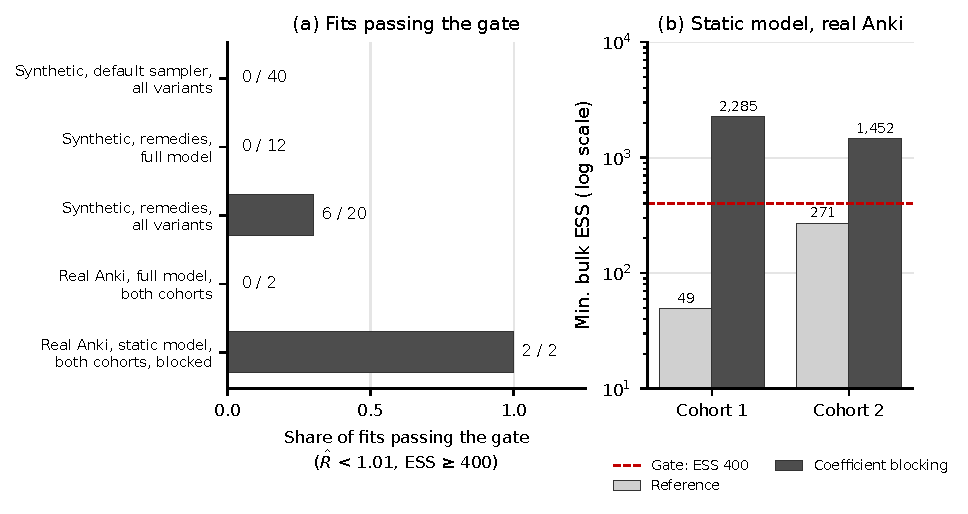
\includegraphics[width=\textwidth]{figures/data/fig_task3_passfail.pdf}
  \caption[Task 3: gate outcomes]{Task 3 sampler study. Left: the share of fits passing the gate for each comparison.
    Right: minimum bulk ESS of the two real static cohorts before and after coefficient blocking, on a logarithmic scale. The
    dashed line is the gate, ESS 400. Every full-model fit fails, and both static cohorts pass after coefficient blocking.}
  \label{fig:fig_task3_passfail}
\end{figure}

The innovation interweaving kernel was designed and implemented as an experimental pilot. No results are available, so none
is reported in this chapter. It is listed as future work in Chapter~\ref{ch:conclusion}.

\section{Computational Cost}
\label{sec:results-cost}

The two benchmarks were run on different hardware. Experiment~2 used a laptop with one core for the Ours fits and eight workers
for the baselines. Experiment~3 ran the proposed model on a Kaggle T4 GPU. Table~\ref{tab:cost} gives the wall-clock
times in seconds, and Figure~\ref{fig:fig_timings} plots the Experiment~2 times on a logarithmic scale. The Experiment~2 fit of the
proposed model took 27,530 seconds, about 7.6 hours, for 2000 sweeps. That is about 13.8 seconds per sweep. The aborted long run took about
15 seconds per sweep. On Duolingo, the GPU fit took 2,598 seconds, and the FSRS-6 (optimised) fit took 688 seconds.

\begin{table}[htbp]
  \centering
  \caption[Wall-clock time]{Wall-clock time in seconds, fit and predict, for each model on each benchmark. A dash means the model
    was not run. Bold marks the lowest value in each column.}
  \label{tab:cost}
  \begin{tabular}{@{}lcccc@{}}
    \toprule
    & \multicolumn{2}{c}{Anki (Experiment 2)} & \multicolumn{2}{c}{Duolingo (Experiment 3)} \\
    \cmidrule(lr){2-3}\cmidrule(lr){4-5}
    Model & Fit & Predict & Fit & Predict \\
    \midrule
    FSRS-6 (default) & \textbf{0} & 99 & \textbf{2.8} & 2,529 \\
    FSRS-6 (optimised) & 653 & 99 & 688 & 2,521 \\
    HLR & 45 & \textbf{0.3} & 235 & \textbf{9} \\
    LagLogit+$\Delta t$ & -- & -- & 894 & 149 \\
    Ours & 27,530 & 1,266 & 2,598 & 1,944 \\
    Ours (+$\kappa$) & 26,130 & 1,340 & -- & -- \\
    \bottomrule
  \end{tabular}
\end{table}

\begin{figure}[htbp]
  \centering
  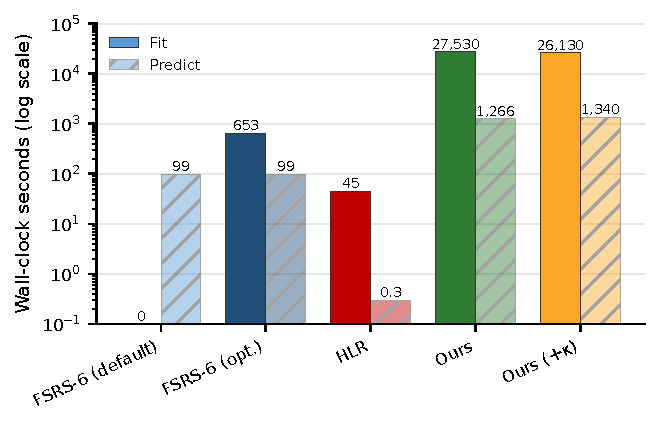
\includegraphics[width=12cm]{figures/data/fig_timings.pdf}
  \caption[Wall-clock time, Experiment 2]{Experiment 2: fit and predict wall-clock time per model, on a logarithmic scale. The
    FSRS-6 (default) fit took 0 seconds.}
  \label{fig:fig_timings}
\end{figure}

Hardware differs between the two benchmarks, so the times are not directly comparable. On Duolingo the proposed model predicted in 1,944 seconds, less than the 2,521 to 2,529 seconds of the FSRS-6 predictions, and its GPU fit took 2,598 seconds.

\section{Summary of Findings}
\label{sec:results-summary}

The main findings of this chapter are as follows.

\begin{enumerate}
  \item Among the five models of Experiment~2 on the Anki benchmark, FSRS-6 with optimised weights has the best log loss, AUC, ECE and calibration; Experiment~4 later adds better models (items 12 to 15). The
    proposed model is better than HLR, with a difference in log loss of $-0.258$ whose interval excludes zero, and worse than both
    FSRS-6 variants, with differences of $+0.043$ and $+0.026$ whose intervals also exclude zero.
  \item Among the five models of Experiment~3 on full Duolingo, the proposed model has the lowest log loss, Brier score, ECE and RMSE over bins, and the
    highest AUC. Its log-loss advantage over FSRS-6 (optimised) is $-0.032$, and over LagLogit+$\Delta t$ it is $-0.023$. These results rest on FSRS-6 (optimised) falling back to default weights for nearly all users, on binary outcomes for both models, and on chains that did not converge (Section~\ref{sec:results-exp3}).
  \item The two benchmarks reverse the ranking of the proposed model and FSRS-6. The reasons are not tested. The candidates are the
    grades, per-user optimisation, the gap range and the data size.
  \item The Duolingo gain over LagLogit+$\Delta t$ comes mostly from the lighter half of users, who supply 55.8\% of the gain from 12.8\% of events. The heaviest quartile supplies 16.8\% of the gain and gains only 0.006 per event, and the median user is slightly worse (Table~\ref{tab:exp3-quartiles}).
  \item In the preliminary Experiment~1, the dynamic model had lower log loss than LagLogit+$\Delta t$ in the 14--60-day bin, and the no-memory variant was not
    distinguishable from the learned rate overall. Experiment~1 used an extract whose provenance is not authenticated, and it is
    not evidence for the model on its own.
  \item The proposed model over-predicts at 61 days and longer on Anki, with a bias of $+0.090$. The model does not remove
    this long-gap error.
  \item On cold cards, the proposed model's AUC is lower than on warm cards, and its gap to FSRS-6 is slightly larger. The cold path is an implementation limitation, and it does not by itself explain the gap.
  \item No run converged for every parameter. No scalar in any run meets the ESS gate of 400, and the learned rate $\lambda$ is the least converged parameter.
    All results are therefore provisional.
  \item The identifiability problems are a $\lambda$--$\sigma^2$ ridge and a rank deficiency of 33 in 37 mean-design columns. The
    Task~3 study finds no full-model fit that passes the gate, and both static real cohorts pass after coefficient blocking.
  \item The cost is high for the sampler on CPU: about 7.6 hours for one Anki fit. The GPU port fits Duolingo in 2,598 seconds.
  \item The interweaving kernel has no results, and it is future work.
  \item In Experiment~4 (Section~\ref{sec:results-exp4}) among the models compared in Experiment~4, the GBDT, which has no memory equation, has the best value of every metric on both Anki and Duolingo. On Anki its log loss is 0.358 against 0.379 for FSRS-6 (optimised), a difference of $-0.021$ whose interval excludes zero. On Duolingo it is 0.259 against 0.300 for FSRS-6 (optimised) and 0.268 for the proposed model (v1). Its lead is largest on Duolingo users with no training rows.
  \item The MAP variants v2 and v3 are level with FSRS-6 (optimised) on Anki, with intervals that include zero, and better than it on Duolingo, but they do not match the proposed model (v1) there. They have no posterior and no convergence diagnostics.
  \item The gain of the GBDT comes mostly from running statistics of the user's own performance and from training on all non-first reviews, not from a memory model. It cannot by itself drive a scheduler, because it has no stability or difficulty state.
  \item Experiment~4 carries disclosed limits: the test set was looked at twice, many variants were tried, a same-session leak was found and fixed, and one seed and one split were used (Section~\ref{sec:results-exp4-disclosures}). The Bayesian model stays the subject of this report, and it is the interpretable one; in these experiments the GBDT is more accurate.
  \item On Duolingo, the smoothed per-user constant floor, which has no memory model, has log loss 0.2723. It beats FSRS-6 (optimised) at 0.3003, the MAP variants, LagLogit+$\Delta t$ and HLR. Only the GBDT (0.2588) and the proposed model (v1, 0.2682) beat it. The margin of v1 is $-0.0040$, with interval $[-0.0045, -0.0035]$. HLR is worse than the global constant on both datasets (Section~\ref{sec:results-exp5-floors}).
  \item On two more Anki samples of 100 users (seeds 1 and 2), the models that were re-run keep the same order. The GBDT has the lowest log loss on each one, and its log loss minus that of FSRS-6 (optimised) is $-0.0210$, $-0.0226$ and $-0.0210$, and each interval excludes zero. The proposed model (v1) was not re-run on these samples (Section~\ref{sec:results-exp5-seeds}).
  \item On the srs-benchmark protocol, with the pooled GBDT trained on other users and evaluated on 1000 users with the benchmark's own folds, the GBDT has unweighted log loss 0.3211, against 0.3580 for FSRS-6 and 0.2860 for RWKV-Instant. Weighted, it is level with RWKV-Curve (0.3143) and behind RWKV-Instant (0.2828). Its boosting reached the 2000-round cap, so this is a lower bound (Section~\ref{sec:results-exp5-srsb}).
\end{enumerate}
